%%%%%%%%%%%%%%%%%%%%%%%%%%%%%%%%%%%%%%%%%%%%%%%%%%%%%%%%%%%%%%%%%%%%%%%%%%%%%%%%%%%%%%%%%%%%%%%%%%%%
% Masters Thesis: A Deep Recurrent Network for Traffic Prediction
% Author: Rabindra Panda
% The University of Melbourne
%%%%%%%%%%%%%%%%%%%%%%%%%%%%%%%%%%%%%%%%%%%%%%%%%%%%%%%%%%%%%%%%%%%%%%%%%%%%%%%%%%%%%%%%%%%%%%%%%%%%

%---------------------------------------------------------------------------------------------------
%	PACKAGES AND OTHER DOCUMENT CONFIGURATIONS
%---------------------------------------------------------------------------------------------------
% The default font size and one-sided printing (no margin offsets)
\documentclass[11pt, oneside]{Thesis}

% Specifies the directory where pictures are stored
\graphicspath{{Figures/}}
% Use the natbib reference package - read up on this to edit the reference style; if you want text
% (e.g. Smith et al., 2012) for the in-text references (instead of numbers), remove 'numbers'
\usepackage[square, numbers, comma, sort&compress]{natbib}
\usepackage{tikz}
\usepackage{multirow}
\usetikzlibrary{trees,shapes,arrows,matrix,chains,positioning,decorations.pathreplacing}

% Colors hyperlinks in blue - change to black if annoying
\hypersetup{urlcolor=black, colorlinks=true}
\title{\ttitle} % Defines the thesis title - don't touch this

\begin{document}

\frontmatter % Use roman page numbering style (i, ii, iii, iv...) for the pre-content pages

\setstretch{1.3} % Line spacing of 1.3

% Define the page headers using the FancyHdr package and set up for one-sided printing
\fancyhead{} % Clears all page headers and footers
\rhead{\thepage} % Sets the right side header to show the page number
\lhead{} % Clears the left side page header

\pagestyle{fancy} % Finally, use the "fancy" page style to implement the FancyHdr headers

\newcommand{\HRule}{\rule{\linewidth}{0.5mm}} % New command to make the lines in the title page

% PDF meta-data
\hypersetup{pdftitle={\ttitle}}
\hypersetup{pdfsubject=\subjectname}
\hypersetup{pdfauthor=\authornames}
\hypersetup{pdfkeywords=\keywordnames}

\clearpage % Start a new page

%---------------------------------------------------------------------------------------------------
%	LIST OF CONTENTS/FIGURES/TABLES PAGES
%---------------------------------------------------------------------------------------------------
% The page style headers have been "empty" all this time, now use the "fancy" headers as defined
% before to bring them back
\pagestyle{empty}
\begin{center}
\begin{tabular}{ l p{8cm}}
  Name & {\authornames} \\
  Student number & 643998 \\
  Supervisor & {\supname} \\
  Total number of credit points & 75 \\
  Type of project & Research \\
  Subject Code & COMP60002\\
  Project title & {\ttitle} \\
\end{tabular}
\end{center}

%---------------------------------------------------------------------------------------------------
%	TITLE PAGE
%---------------------------------------------------------------------------------------------------

\begin{titlepage}
\begin{center}

\includegraphics[scale=0.3]{unilogo.pdf} % University/department logo - uncomment to place it

\textsc{\LARGE \deptname}\\ % Department name
\textsc{\LARGE \univname}\\[1.5cm] % University name
\textsc{\Large Masters Thesis}\\[0.5cm] % Thesis type

\HRule \\[0.4cm] % Horizontal line
{\huge \bfseries \ttitle}\\[0.4cm] % Thesis title
\HRule \\[1.5cm] % Horizontal line

\begin{minipage}{0.4\textwidth}
\begin{flushleft} \large
\emph{Author:}\\
% Author name
\href{http://www.rabipanda.com}{\authornames}
\end{flushleft}
\end{minipage}
\begin{minipage}{0.4\textwidth}
\begin{flushright} \large
\emph{Supervisor:} \\
% Supervisor name - remove the \href bracket to remove the link
\href{http://www.cis.unimelb.edu.au/people/staff.php?person_ID=618008}{\supname}
\end{flushright}
\end{minipage}\\[3cm]

 % University requirement text
\large \textit{A thesis submitted in fulfilment of the requirements\\ for the degree of
\degreename}\\[0.3cm]

%\textit{in the}\\[0.4cm]
%\groupname\\
%\deptname\\[2cm] % Research group name and department name

{\large \today}\\[4cm] % Date
\vfill
\end{center}

\end{titlepage}

%---------------------------------------------------------------------------------------------------
%	DECLARATION PAGE
%---------------------------------------------------------------------------------------------------

\Declaration{

\addtocontents{toc}{\vspace{1em}} % Add a gap in the Contents, for aesthetics

I , \authornames, certify that

\begin{itemize}

\item[\tiny{$\blacksquare$}] this thesis does not incorporate without acknowledgement any material
previously submitted for a degree or diploma in any university; and that to the best of my knowledge
and belief it does not contain any material previously published or written by another person where
due reference is not made in the text.

\item[\tiny{$\blacksquare$}] where necessary I have received clearance for this research from the
University's Ethics Committee and have submitted all required data to the Department.

\item[\tiny{$\blacksquare$}] the thesis is approximately 20000 words in length (excluding text in
images, table, bibliographies and appendices).
\end{itemize}

Signed:\\
\rule[1em]{25em}{0.5pt} % This prints a line for the signature

Date:\\
\rule[1em]{25em}{0.5pt} % This prints a line to write the date
}

\clearpage % Start a new page


%---------------------------------------------------------------------------------------------------
%	ABSTRACT PAGE
%---------------------------------------------------------------------------------------------------

\setstretch{1.3} % Reset the line-spacing to 1.3 for body text (if it has changed)

\abstract{\addtocontents{toc}{\vspace{1em}}
Road traffic congestion is a global issue that results in significant wastage of time and resources.
Rising population, urbanisation, growing economies and affordable personal vehicles aggravate the
issue. In Australia, across Melbourne and Sydney, people on average spent 35\% more travel
time\footnote{TomTom Traffic Index.} during congestion. Many urban cities have been trying to
mitigate this issue by expanding and modernising the transporation infrastructure. Even though
increasing the capacity accomodates the traffic demand, studies have shown this does not eliminate
the congestion problem. Hence, since 1970's advanced traffic management systems have been used to
address this. But for these systems to increase their operational efficiencies and fully realise
their effectiveness, they need to have the predictive capabilities in the short term, usually
ranging between few seconds to few hours. The research in short term traffic prediction has been
active since the 1970's. Numerous models have been proposed to use the traffic data collected by
inductive loop detectors for short term traffic prediction. Most of the works have shown promising
results through experiments at particular locations, however we are still to find a robust and
globally adaptable solution. In last decade the attention have shifted from theroitically well
established parametric methods to non parametric data driven algorithms. This work is an extension
to that. Neural networks have always been one of the most capable mathematical models that can model
complex non-linear relations. Upto 2006, their use have been hindered by practical issues related to
the training. But recent breakthroughs in new ways of training deep neural architecture have made
them reemerged as victors by realising the capabilities the had promised. In this thesis we study
and extend their application to short term traffic predictions. We used a deep Long Short Term Memory
neural network to predict the short term traffic volumes at a network level. We used the volume data
collected by Vicroads in Melbourne. We compared the results of our work with several existing
methods and found some promising results.
}
\clearpage % Start a new page

%---------------------------------------------------------------------------------------------------
%	ACKNOWLEDGEMENTS
%---------------------------------------------------------------------------------------------------

\setstretch{1.3} % Reset the line-spacing to 1.3 for body text (if it has changed)

\acknowledgements{\addtocontents{toc}{\vspace{1em}} % Add a gap in the Contents, for aesthetics

I am deeply indebted to the following people for their invaluable support and comments without which
I would not have been able to complete this work\ldots
}
\clearpage % Start a new page

%---------------------------------------------------------------------------------------------------
%	LIST OF CONTENTS/FIGURES/TABLES PAGES
%---------------------------------------------------------------------------------------------------
% The page style headers have been "empty" all this time, now use the "fancy" headers as defined
% before to bring them back
\pagestyle{fancy}

\lhead{\emph{Contents}} % Set the left side page header to "Contents"
\tableofcontents % Write out the Table of Contents

\lhead{\emph{List of Figures}} % Set the left side page header to "List of Figures"
\listoffigures % Write out the List of Figures

\lhead{\emph{List of Tables}} % Set the left side page header to "List of Tables"
\listoftables % Write out the List of Tables

%---------------------------------------------------------------------------------------------------
%	ABBREVIATIONS
%---------------------------------------------------------------------------------------------------

\clearpage % Start a new page

\setstretch{1.5} % Set the line spacing to 1.5, this makes the following tables easier to read

\lhead{\emph{Abbreviations}} % Set the left side page header to "Abbreviations"
\listofsymbols{ll} % Include a list of Abbreviations (a table of two columns)
{
\textbf{ARIMA} & \textbf{A}uto \textbf{R}egressive \textbf{I}ntegrated \textbf{M}oving \textbf{A}verage \\
\textbf{LSTM} & \textbf{L}ong \textbf{T}erm \textbf{S}hort \textbf{M}emory \\
\textbf{RNN} & \textbf{R}ecurrent \textbf{N}eural \textbf{N}etwork \\
\textbf{SCATS} & \textbf{S}ydney \textbf{C}oordinated \textbf{A}daptive \textbf{T}raffic \textbf{S}ystems \\
}

%---------------------------------------------------------------------------------------------------
%	NOTATIONS
%---------------------------------------------------------------------------------------------------

%\clearpage % Start a new page
%
%\lhead{\emph{Notations}} % Set the left side page header to "Notations"
%
%\listofnomenclature{ll} % Include a list of Symbols (a two column table)
%{
%% Symbol & Name \\
%$y$ & Scalar value \\
%$\textbf{x}$ & Vector \\
%$\textbf{M}$ & Matrix \\
%$\Sigma$ & Covariance matrix \\
%}

%---------------------------------------------------------------------------------------------------
%	DEDICATION
%---------------------------------------------------------------------------------------------------

\setstretch{1.3} % Return the line spacing back to 1.3

\pagestyle{empty} % Page style needs to be empty for this page

\dedicatory{Dedicated to\ my parents and teachers}% Dedication text

\addtocontents{toc}{\vspace{2em}} % Add a gap in the Contents, for aesthetics

%---------------------------------------------------------------------------------------------------
%	THESIS CONTENT - CHAPTERS
%---------------------------------------------------------------------------------------------------

\mainmatter % Begin numeric (1,2,3...) page numbering

\pagestyle{fancy} % Return the page headers back to the "fancy" style

% Include the chapters of the thesis as separate files from the Chapters folder Uncomment the lines
% as you write the chapters


% Chapter 1

\chapter{Introduction} % Main chapter title

\label{Chapter1} % For referencing the chapter elsewhere, use \ref{Chapter1}

% This is for the header on each page - perhaps a shortened title
\lhead{Chapter 1. \emph{Introduction}}

% Quotation
{``As a reader I loathe introductions...Introductions inhibit pleasure, they kill the joy of
anticipation, they frustrate curiosity."}
\begin{flushright}
Harper Lee, \textit{To Kill a Mockingbird} (1960)
\end{flushright}

\section{Background}
Predicting the future has always been a fascinating topic throughout the history of mankind.
Instances of predicting the future through unconventinal means have been mentioned in various
forms of literature such as mythologies, fantasy, science fiction etc. Even today, while the
means of prediction have changed, we still try to predict almost everything in our day to day
lives - from election polls to sports outcomes to financial results.

Road traffic congestion is a serious global issue, resulting in significant wastage of time and
resources. Several factors such as growth in population, urbanisation and affordable personal vehicles
have aggravated theh issue. In Australia the number of personal vehicles have grown from 1.4 million
to 13 million during the period from 1955 to 2013, an average annual growth of 4\%\footnote{Australian
Bureau of Statistics - \url{http://www.abs.gov.au/AUSSTATS/abs@.nsf/Lookup/4102.0Main+Features40July+2013}}.
In 2012, the majority of Australians used personal vehicles, 72\% to work or study and 88\% for other activities.
When it comes to travel time, across Sydney and Melbourne, the overall travel time is 37\% and 29\% more beacuse of
congestion\footnote{TomTom Traffic Index - \url{http://www.tomtom.com/en_au/trafficindex/list}}.
Across the globe, this figure is far worse in many other cities like Mexico City(59\%), Bangkok(57\%),
Istanbul(50\%), Rio de Janiro(47\%) and Moscow(44\%). While improving and extending the road infrastructure has
reduced the issue to some extent, this is time consuming and does not eliminate the issue.
Thus in last few decades, for better planning and control of road traffic, advanced traffic
management systems have been deployed around the world. Still the role of these systems is not
fully realised without predictive capabilities in the short term, without which these systems only
react to events at real time. While this is the desired objective, the performance of these systems
could be significantly improved by making them proactive(\citet{smith1997traffic}). Short term traffic
flow prediction is not only helpful for these advanced traffic control systems, it is also useful
for advanced traveller information systems.


Research in short term traffic prediction had been active for more than threee decades. This shows the
strong interest in solving the growing problem of traffic congestion by providing accurate predictions
that can be used in both advanced traffic management systems and adavanced traveller information systems.
However due to the complex nature of traffic conditions, a globally applicable short term prediction
model, that can be easily embedded into advanced traffic management and advanced traveller information
systems, is yet to be found.

Neural networks have the potential to solve such complex problems, and it has been realised long term
ago. But due to the practical issue that arise in training, ther use have been restricted. In last
decade new ways of training deep neural networks have made them reemerges as victors. Also the use
of fast graphical processing units have reduced the training time by 10 to 20 times. The capabilities
that neural networks had initally promised have been realised in several fields such as machine
vision, image and speech recognition, natural language processing etc. In this study we extend their
applications to the fiels of short term traffic predictions. We use several variants of deep recurrent
neural networks and suggest a deep LSTM network to model the traffic conditions and make predictions
at multiple steps ahead at a network level. Our study shows some promising results and encourages
similar future works.


\section{Motivations}
There are two main factors that have motivated us to undertake this study. These are

\begin{itemize}
\item Short term traffic prediction has more than three decades of active research, making this a
challenging task. This is mainly due to the complex nature of traffic data - temporal and spatial
relationships, noise and missing values, effects of non-recurrent events (weather, accidents,
public events etc.)

\item Availability of huge amount of historical data and new breakthroughs in deep learning.

\end{itemize}

\section{Objectives and scope}

\textbf{Research objective} is to use the large amount of available historical traffic volume data and
apply deep neural networks for future predictions at a network level. More importantly this research
tries to answer the following questions -

\begin{itemize}
\item How can we use the large amount of traffic data available for predicting short term traffic
 flow for better predictions?
\item Can we use the ability of deep neural networks to capture the tempo-spatial dimension of
traffic conditions and make predictions at a transportation network level?
\end{itemize}

\textbf{Research scope} - The scope of this research is to predict traffic volume in the
short term. The use of the phrase 'short term' implies that we are only interested in the
prediction within a very short horizon which typically ranges between few seconds to few
hours in practice. The traffic parameters that are of usually of interest to be predicted are
volume, time, speed and density. The scope of this research is limited to the prediction of only
traffic volume. While doing so, we are only taking the past data into consideration and not
taking the non-recurrent phenomena such as traffic accidents, weather or public events into
consideration.


\section{Thesis outline}

\textbf{Chapters} -- This thesis is divided into six chapters.

\begin{itemize}
\item Chapter 1: Introduction - In this chapter we present the background and research context,
research objectives and scope.

\item Chapter 2: Traffic Prediction: Literature Review - In this chapter we provide a reasonably
thorough review of existing literature on short term traffic prediction.

\item Chapter 3: SCATS Traffic Volume Data - In this chapter we describe the traffic volume data
collected by VicRoads using the SCATS systems. Methods to deal with missing data are presented in
this chapter. Finally we present some exploratory data analysis on the traffic data.

\item Chapter 4: A Deep LSTM Network for Short Term Traffic Prediction - In this chapter we propose
a long short term memory (LSTM) neural network model for short term traffic prediction.

\item Chapter 5: Evaluation of the Model - In this chapter we evaluate the model and compare the results
with existing methods.

\item Chapter 6: Conclusions and Future Directions - In this chapter we conclude our thesis and
provide inputs for future work.
\end{itemize}

% Chapter 2

% Main chapter title
\chapter{Traffic Prediction: Literature Review}

% For referencing the chapter elsewhere, use \ref{Chapter2}
\label{Chapter2}

% This is for the header on each page - perhaps a shortened title
\lhead{Chapter 2. \emph{Traffic Prediction: Literature Review}}

% Quotation
{``There is no way that we can predict the weather six months ahead beyond giving the seasonal
average"}
\begin{flushright}
Stephen Hawking, \textit{Black Holes and Baby Universes} (1993)
\end{flushright}

%---------------------------------------------------------------------------------------------------
%	CONTENT
%---------------------------------------------------------------------------------------------------
\section{Introduction}
%\cite{ahmed1979analysis,van2012short,vlahogianni2004short,vlahogianni2014short,smith1997traffic}
In this chapter we provide a reasonably complete review of existing literature on short term
traffic flow prediction. Research on short term traffic prediction has been going on since 1979,
\citet{ahmed1979analysis}. After more than three decades of research, short term traffic flow
prediction is still an interesting reserch subject for many professionals around the world. The
simplest reseaon being the complex non-linear nature of traffic data and the effects of
non-recurrent events(weather, public events, accidents etc.) on it.  Critical reviews of existing
literature on short term traffic flow have been presented in detail by \citet{smith1997traffic},
\citet{vlahogianni2004short}, \citet{van2012short} and \citet{vlahogianni2014short}. The use of
the phrase 'short term' limits the scope of traffic prediction in terms of the prediction horizon
which usually varies between few seconds to few hours depending upon the approach and application.

The traffic parameter that are predicted can be - flow(number of vehicles per hour), time(minutes
to travel between two points), speed(mean speed in km/hour) and density(number of vehicles per km).

Selecting the right model for short term traffic prediction is a challenging task. A number of
models have been suggested and yet there is no one-fits-all model. The various methods that have
been suggested for short term traffic prediction can be categorised into four groups -
naive, parametric, non-parametric and hybrid as shown in figure \ref{fig:taxonomyTrafficPrediction}.


\begin{figure}
\centering
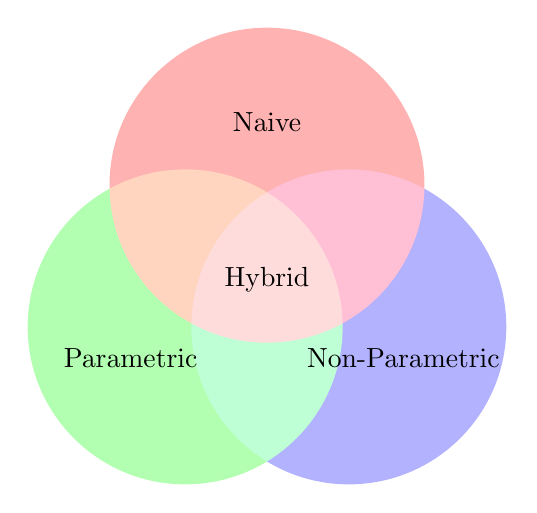
\begin{tikzpicture}
  \begin{scope}[blend group = soft light]
    \fill[red!30!white]   ( 90:1.2) circle (2);
    \fill[green!30!white] (210:1.2) circle (2);
    \fill[blue!30!white]  (330:1.2) circle (2);
  \end{scope}
  \node at (90:2)    {Naive};
  \node at (210:2)   {Parametric};
  \node at (330:2)   {Non-Parametric};
  \node              {Hybrid};
\end{tikzpicture}
\caption{Methods used for short term traffic prediction} \label{fig:taxonomyTrafficPrediction}
\end{figure}

\section{Naive methods}
These methods, while called as naive are  sometimes used in practice because of the simplicity
of the method and the ease of implementation. In most cases these methods are used as baselines
for comparison while creating more advances methods. The simplest naive approach in short term
prediction would be to take the last observed value and this involves no computational effort.

Instanteneous Travel Time(ITT) assumes that the traffic conditions will remain constant indefinitly.

Historical averages uses the average of past observed values.

\section{Parametric models}
In parametric models, we estimate the parameters from the training dataset to determine the
function that classifies new unseen data. The number of parameters are fixed. The advantage of
parametric models are that these perform quite well in situations where the large amount of data
is not available. Some of the typical examples of parametric models include Linear and
nonlinear regression, ARIMA models, Kalman filter, Linear SVM etc.

\subsection{Linear and nonlinear regression}
In machine learning and statistical applications, the use of linear models are predominant. These
models are also important in time series domains such as traffic flow prediction. The primary
idea behind the regression is to express the output variable as a linear combination of input
vectors. We can express the linear regression in time series as an ouput influenced by a
collection of inputs, where the inputs could possibly be an independent series

        \begin{equation}
            x_{t} = \beta_{1}z_{t1} + \beta_{2}z_{t2} + ... + \beta_{q}z_{tq} + w_{t}
        \end{equation}

where $ \beta_{1}, \beta_{2},...,\beta_{q} $ are unknown regression coeffiecients and $w_{t}$ is
a random error.

\citet{hogberg1976estimation} used non-liner regression for traffic prediction.

\subsection{ARIMA}
%  Introduction to ARIMA models
% \citet{chen2011short,kumar2015short,min2009short,min2010urban,szeto2009multivariate,
%  van1996combining,williams2001multivariate,williams2003modeling}

ARIMA(Auto Regressive Integrated Moving Average) is a class of parametric regression models. In
this section we will introduce ARIMA and related methods such as exponential smoothing and moving
averages. For an in depth understanding of these models the reader is encouraged to refer to to
~\citet{tong1990non}, ~\citet{brockwell2006introduction} and ~\citet{box2015time}. It is
important to understand that ARIMA modelling works only with stationary time series data. A
stationary time series is one whose properties do not depend on the time it is being observed.
Trends and seasonality affect time series and hence make it non-stationary. Although this seems as a
big restriction, in short term traffic prediction, ARIMA models have been very successful. Two
basic models constituate ARIMA models - AR(autoregressive) and MA(moving average).

The main idea behind autoregressive models is that past values affect the present value, i.e.
$x_{t}$ can be expressed as a function of past p values $ x_{t-1}, x_{t-2},...,x_{t-p} $ , where
p is the number of steps into the past. We can express an autoregressive model of order p as below

        \begin{equation} \label{eq:autoregressive}
          x_{t} = \phi_{1}x_{t-1} + \phi_{2}x_{t-2} + ... + \phi_{p}x_{t-p} + w_{t}
        \end{equation}

where $x_{t}$ is stationary and $\phi_{1}, \phi_{2},..., \phi_{p}$ are constant
parameters that are to be chosen. We have added the term $w_{t}$ as a Guassian white noise with
zero mean and variance $\sigma^{2}_{w}$.

In the MA model, the current value is dependent on the last q one-step forecast errors
$e_{t-1}, e_{t-2},...,e_{t-q}$ and the white noise $w_{t}$. The expression for moving average
is

        \begin{equation} \label{eq:movingaverage}
          x_{t} = -\theta_{1}e_{t-1} - \theta_{2}e_{t-2} - ... - \theta_{q}e_{t-q} + w_{t}
        \end{equation}

$\theta_{1}, \theta_{2},..., \theta_{q}$ are the parameters to be chosen.

Now proceeding to an ARMA(autoregressive moving average) model, we define an ARMA(p,q) model
where the present value $x_{t}$ is dependent on p past recent values and q past recent forecast
errors and a white noise $w_{t}$.

        \begin{equation} \label{eq:arma}
          x_{t} = \phi_{1}x_{t-1} + \phi_{2}x_{t-2} + ... + \phi_{p}x_{t-p} - \theta_{1}e_{t-1}
          - \theta_{2}e_{t-2} - ... - \theta_{q}e_{t-q} + w_{t}
        \end{equation}

When q is 0, the model becomes an autoregressive model of order p, AR(p) and when p is 0 the model
is a moving average of order q, MA(q). We can rewrite \ref{eq:arma} by using the backshift
operator $B^{\alpha}$, which is defined as $B^{\alpha}z_{t} = z_{t-\alpha}$,

        \begin{equation} \label{eq:armarewrite}
          \phi(B)x_{t} = \theta(B)e_{t}
        \end{equation}

where
        \begin{equation}
            \phi(z) = 1 - \phi_{1}z - ... - \phi_{p}z^{p}
        \end{equation}
        \begin{equation}
            \theta(z) = 1 - \theta_{1}z - ... - \theta_{q}z^{q}
        \end{equation}

In practice, most time series data are non-stationary and so several approaches, for instance
by differencing, are taken to make it stationary before applying the ARMA(p,q) model. By
combining differencing with autoregressive and moving average we obtain the ARIMA model defined
as below
        \begin{equation} \label{eq:arima}
          x'_{t} = \phi_{1}x'_{t-1} + \phi_{2}x'_{t-2} + ... + \phi_{p}x'_{t-p} -
          \theta_{1}e_{t-1} - \theta_{2}e_{t-2} - ... - \theta_{q}e_{t-q} + w_{t}
        \end{equation}

where $x'_{t}$ is the differenced series. Formally the model is denotes as ARIMA(p,d,q) where p
is the order of autoregressive part, d is the degree of differencing and q is the order of moving
average. This is also known as a non-seasonal ARIMA model.

The common method used to determine the parameters in an ARIMA(p,d,q) model is known as the
Box-Jenkins approach (\citet{box2015time}) which is three stage procedure. The three stages are
identification, estimation and diagnostic checking. At the identification stage, the values p, d
and q are determined by observing the autocorrelation and partial autocorrelation functions of
the time series and its differences. At the estimation stage, the maximum liklihood estimates are
determined for each model parameter. Finally in the dignostics stage, the residuals are analysed
and model comparisions are done. If the model fits well then the standardised residuals behave as
an i.i.d. with mean zero and variance one.

% Application in traffic forecast
\citet{ahmed1979analysis} used Box-Jenkins method for short-term traffic forecast. The input data
used was 166 sets of time series traffic data collected by freeway traffic surveillance systems in
three locations - Los Angeles, Minneapolis and Detroit. The authors concluded an ARIMA(0,1,3) model
as a resonable fit for the short term prediction task.

\citet{nihan1980use} used the Box-Jenkins technique on monthly data collected on a freeway segment
from 1968 to 1976.

\citet{kumar2015short} used a seasonal ARIMA in a context of limited data for short term traffic 
prediction.

% Conclusions - pros and cons
The major defficiency of tha ARIMA models is that they do not take the extremes into
consideration and focus on the means. This is in contrast to the nature of the traffic data.
ARIMA models are also have the inability to perform will with missing data as pointed out by
\citet{smith1997traffic}.

\subsection{Kalman filter}
% \citet{guo2010real,guo2014adaptive,okutani1984dynamic,wang2005real,xie2007short}
\citet{okutani1984dynamic} used Kalman filtering in traffic prediction in an urabn network and
extended it for freeways.

The main advantage of Kalman filtering is the state variable is updated continuously.

\subsection{Other parametric models}

\section{Non-Parametric models}
In nonparamtric models the parameters are not fixed, and vary with the amount of data available.
Usually more data is required for this models than parametric models. The advantage of these models
is that they can model the complex non-linear data better. Some of the widely used non-parametric
models are - k-Nearest Neighbour, Non-parametric regrssion and Neural Networks

\subsection{K-nearest neighbour}
% \citet{lv2009real,myung2011travel,zhang2013improved} \citet{meng2015two}

The basic process of the k-nearest neighbour algorithm is described in figure
\ref{fig:KnnProcessFlow}.

\tikzstyle{block} = [rectangle, draw, text width=5em, text centered, rounded corners,
minimum height=4em]
\tikzstyle{line} = [draw, -latex']
\tikzstyle{cloud} = [draw, ellipse, node distance=4cm, minimum height=3em]

\begin{figure}
\centering
\begin{tikzpicture}[node distance = 3cm, auto]
    % Place nodes
    \node [block] (pp) {Preprocess Data};
    \node [cloud, left of=pp] (hd) {Historical data};
    \node [cloud, right of=pp] (rd) {Real-time data};
    \node [block, below of=pp] (msv) {Match state vector};
    \node [block, below of=msv] (knn) {K nearest neighbour};
    \node [block, left of=knn, node distance=3cm] (prd) {Predictions};
    % Draw edges
    \path [line] (pp) -- (msv);
    \path [line] (msv) -- (knn);
    \path [line] (knn) -- (prd);
    \path [line,dashed] (hd) -- (pp);
    \path [line,dashed] (rd) -- (pp);
\end{tikzpicture}
\caption{K nearest neighbour process flow} \label{fig:KnnProcessFlow}
\end{figure}

\subsection{Fuzzy logic}
% \cite{zhang2008short}

\subsection{Bayesian networks}
% \cite{castillo2008predicting}

\subsection{Neural networks}
% \cite{adeli2001neural,abu2011modeling,bengio1994learning,boto2010wavelet,chan2012neural,
% chan2012optimization,chan2013prediction,chen2001study,dia2001object,dougherty1997short,
% haykin2009neural,hochreiter2001gradient,hodge2014short,hosseini2012short,
% innamaa2005short,ishak2004optimizing,jiang2005dynamic,karlaftis2011statistical,kirby1997should,
% qiu2011bayesian,sun2012network,van2005accurate,vlahogianni2005optimized,
% vlahogianni2007prediction,vlahogianni2013testing,yasdi1999prediction,zheng2006short}
\label{subsec:neuralNetworksTrafficPred}
Artificial Neural Networks(ANN) were mathematical models (\citet{mcculloch1943logical},
\citet{rosenblatt1958perceptron}) designed to  provide a representation of how the human brain
works. It is obvious now that these mathematical models bear little resemblance to the structure
of brain, yet they have been hugely successful. Because they were initially inspired by the
biological brain, the term neural is associated with such kind of mathematical models. A basic
artificial neural network consists of a set of nodes connnected by edges with weights. We can say
that the nodes represent the biological neurons and the edges represent the synapses. The
conections among the nodes can be cyclic or acyclic. The former is known as a feedforward neural
network and the later as a recurrent network. We describe about these neural networks in more
details in chpater \ref{Chapter4}.

Several variations of artificial neural networks have been used in short term traffic prediction.
Some well known examples include - \textit{Multilayer perceptrons, Radial basis function
networks, Kohnen maps} and \textit{Hopfield networks}.


\subsection{Other nonparametric models}

\section{Hybrid Methods}
% \cite{alecsandru2003hybrid,alecsandru2004hybrid,chan2012neural,chen2001study,dimitriou2008adaptive,
% hong2011hybrid,mccrea2010hybrid,wang2013short,xiang2010new,zeng2008short,zhang2014hybrid}


\section{Comparisons}

% Chapter 3

\chapter{SCATS Volume Data} % Main chapter title

% For referencing the chapter elsewhere, use \ref{Chapter3}
\label{Chapter3}

% This is for the header on each page - perhaps a shortened title
\lhead{Chapter 3. \emph{SCATS Volume Data}}

%----------------------------------------------------------------------------------------
% Quotation
``There is no order in the world around us, we must adapt ourselves to the requirements of chaos
instead."

\begin{flushright}
Kurt Vonnegut, \textit{Breakfast of Champions} (1973)
\end{flushright}

%---------------------------------------------------------------------------------------------------
%	CONTENT
%   Reference - http://www.scats.com.au/files/an_introduction_to_scats_6.pdf
%---------------------------------------------------------------------------------------------------
\section{Introduction}
SCATS(Sydney Coordinated Adaptive Traffic System) is an adaptive traffic control system. It was
developed by the Department of Main Roads in the 1970's. SCATS operates in real-time by adjusting
signal timings in response to changes in traffic demand and road capacity. All major and minor
cities in Australia and New Zealand use SCATS. Few other cities around the world such as Hong
Kong, Kuala Lumpur, Sanghai and Singapore also have adopted SCATS over other adaptive traffic
control system. In Melbourne and surrounding cities, SCATS controls more than 3,900 sets of traffic
signals

There are three main parameters that SCATS user to achieve traffic signal coordination:
\begin{itemize}
\item[\tiny{$\blacksquare$}] Cycle time: The total time of all signal sequences in a cycle
\item[\tiny{$\blacksquare$}] Phase split: The proportion of the cycle time allocated to each phase
\item[\tiny{$\blacksquare$}] Offset: The time relationship between the starting and finishing of
the green phases of succesive sets of signals within a coordinated system
\end{itemize}

The desicion making of the SCATS system occurs at two levels - \emph{strategic} and \emph{tactical}.


\section{Volume data}
Traffic loop detectors are embedded in the raod pavement and located in each lane near the stop
line at traffic intersections. These detectors collect traffic volume and the time it takes a
vehicle to clear the loop.


\subsection{Handling missing data}


\section{Exploratory analysis}
Figure \ref{fig:AverageTrafficVolume} shows the daily, weekly, monthly and yearly average traffic
volume at a site location.Figure \ref{fig:TypicalDayTraffic} shows how a typical day of the week
on average looks like at a site location.

\begin{figure}[htbp]
  \centering
    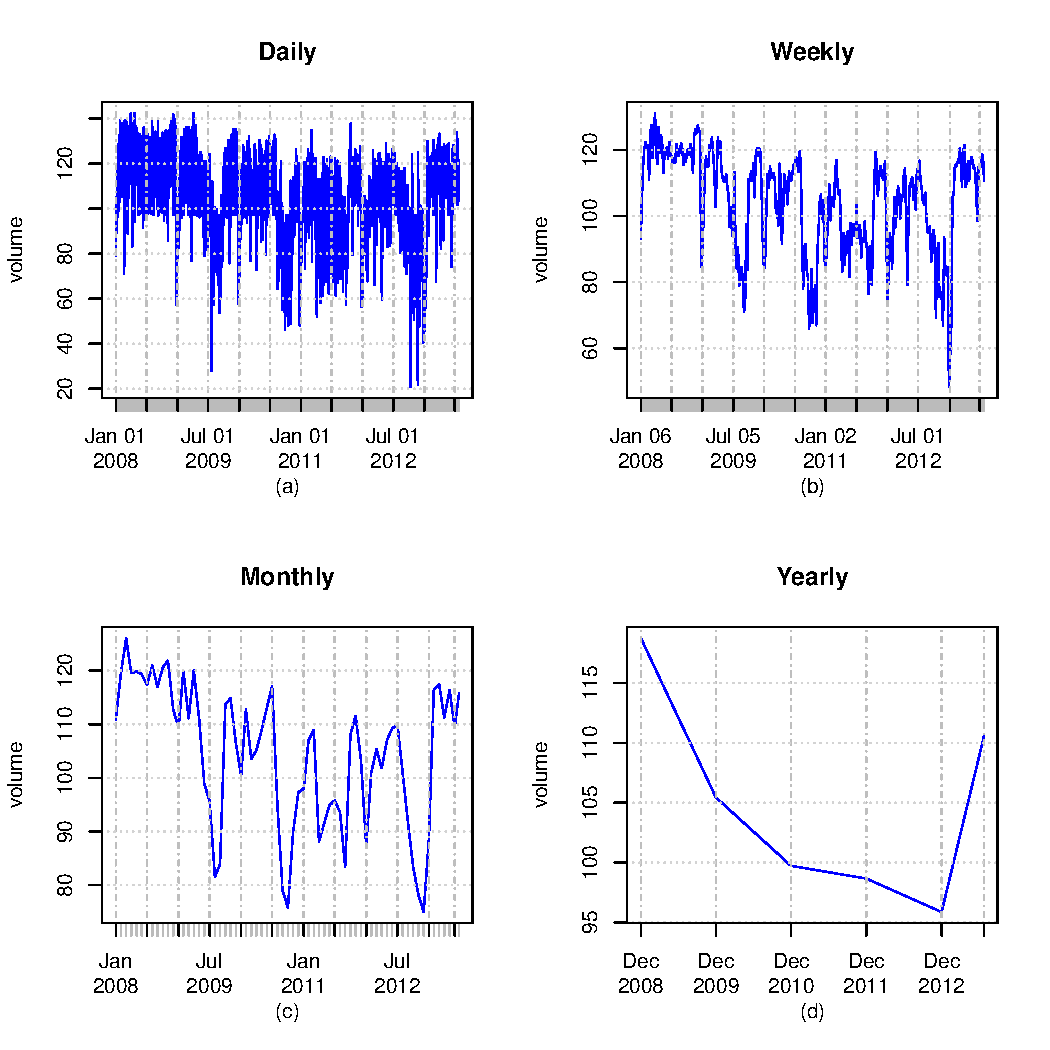
\includegraphics[width=\textwidth,height=\textheight,keepaspectratio]{Figures/averages.pdf}
    \rule{35em}{0.5pt}
  \caption[Average Traffic Volume]{(a) daily, (b) weekly, (c) monthly and (d) yearly average of
  traffic volume (15 mins interval) at a site location from the period 01/01/2008 to 26/07/2013}
  \label{fig:AverageTrafficVolume}
\end{figure}

\begin{figure}[htbp]
  \centering
    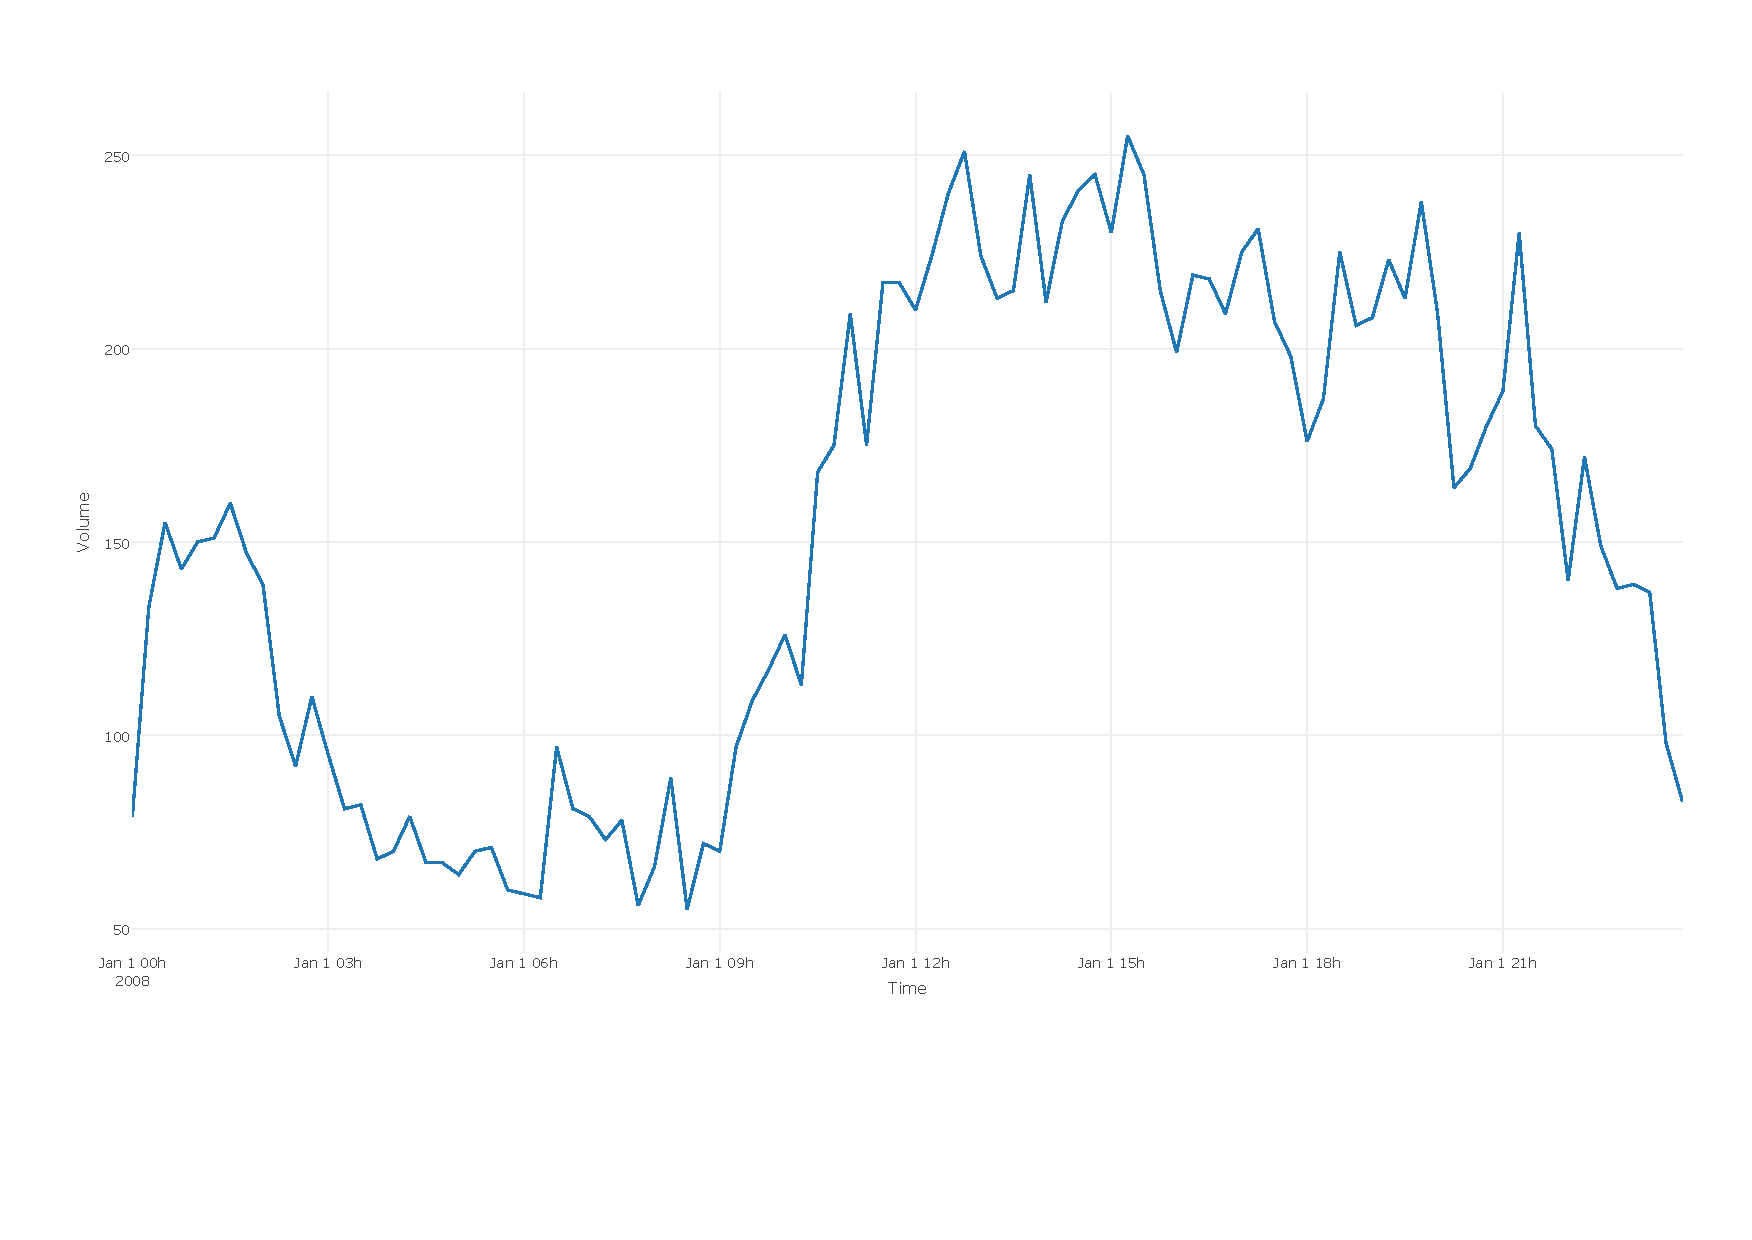
\includegraphics[width=\textwidth,height=\textheight,keepaspectratio]{Figures/typical-day.pdf}
    \rule{35em}{0.5pt}
  \caption[Average traffic on each day of the week]{Shows how a typical day of the week on
  average looks like at a site locationat a site location from the period 01/01/2008 to 26/07/2013}
  \label{fig:TypicalDayTraffic1}
\end{figure}

\begin{figure}[htbp]
  \centering
    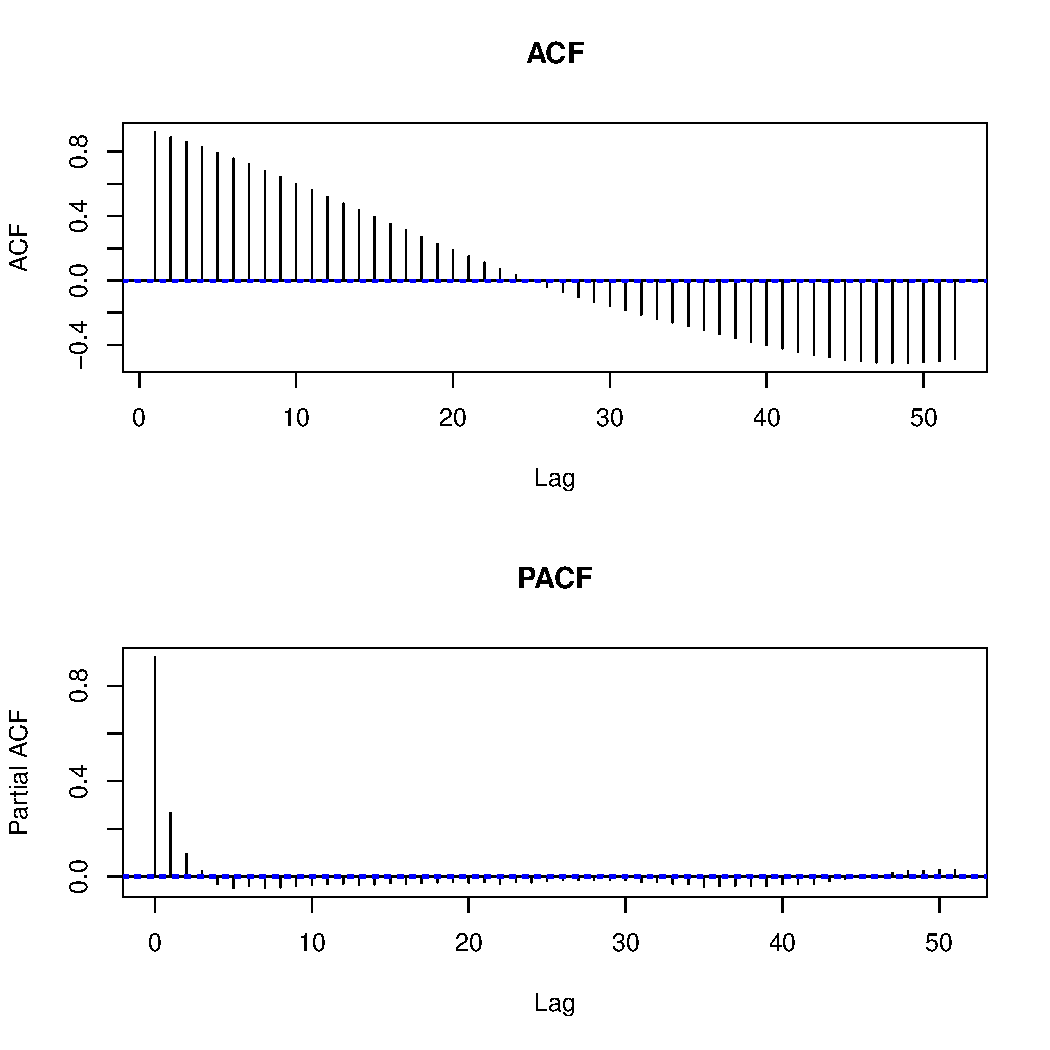
\includegraphics[width=\textwidth,height=\textheight,keepaspectratio]{Figures/acf-pacf.pdf}
    \rule{35em}{0.5pt}
  \caption[Plots of ACF and PACF]{Shows how a typical day of the week on
  average looks like at a site locationat a site location from the period 01/01/2008 to 26/07/2013}
  \label{fig:TypicalDayTraffic1}
\end{figure}



% Chapter 4

\chapter{A Deep LSTM Network for Short Term Traffic Prediction} % Main chapter title

\label{Chapter4} % For referencing the chapter elsewhere, use \ref{Chapter4}

% This is for the header on each page - perhaps a shortened title
\lhead{Chapter 4. \emph{A Deep LSTM Network for Short Term Traffic Prediction}}

% Quotation
{``I am a brain, Watson. The rest of me is a mere appendix."}
\begin{flushright}
Arthur Conan Doyle, \textit{The Adventure of the Mazarin Stone} (1921)
\end{flushright}

%---------------------------------------------------------------------------------------------------
%	CONTENT
%  \cite{bengio2015deep,graves2013generating,hochreiter2001gradient,bengio1994learning,
%       gers2000learning,hochreiter1997long}
%  \cite{busseti2012deep} \cite{karpathy2015visualizing} \cite{graves2012supervised}
% \cite{bishop2007pattern} \cite{gers2001long}
%---------------------------------------------------------------------------------------------------

In section \ref{subsec:neuralNetworksTrafficPred}, we presented a brief introduction to artificial
neural networks and reviewed existing literature in short term traffic prediction that used
various types of neural networks. In the following sections we present a bried overview of deep
learning. We then describe deep feedforward networks, deep recurrent networks with emphasis on
the Long Short Term Memory(LSTM) networks which are a redesigned version of recurrent networks.
Later we present how we can we can use these kind of networks for short term traffic prediction.

\section{Introduction}
Today we live in a world where almost every interaction of ours with the external world uses some
form of computing. Computers have become an inseparable part of human lives. In the earlier days
when computers were built, people began to ponder whether they could achieve human level
of intelligence. Even though at that point the answers seemed optimistic, it has taken quite
some time and understanding on our part to make significant achievements in the field of
artificial intelligence. One of the approaches was to use knowldge base systems, where computers
reason about real world concepts, that were defined in hard-coded formal langauges, using logical
inference rules. These systems led to little success. The difficulties faced in the knwoledge
based appproach made us built computers to learn automatically from data, an approach we know as
machine learning.

A large number of real world problems could eaily be tackled using machine leraning. However for
the machine learning algorithms to perorm well they need to be provided with proper representaion
of data. For example, in a problem where we would like to detect humans in images, it is
difficult to represent various shapes of human body in terms of raw pixels. Finding a proper
representation from data is a challenge and sometimes become very difficult. A class of machine
learning algorithms called representation learning, tackles this problem by learning the
representaions as well. Autoencodes are such types of algorithms. Again the problem with
representation learing is that it is not easy to find the representations due to the presence of
various factors of influence (\citet{bengio2015deep}). Deep learning solves this problem in
representation learning by taking a layered approach by expressing representations in terms of
simpler representations. The mapping from the input to output is done through a series of hidden
layers, where each layer is an abstraction on the previous layer. The depth of the model can be
viewed as the depth of the computational graph, i.e. the number of sequential instructions that
need to be executed to map an input to output.

\section{Deep feedforward networks}
Deep feedforward networks are the most important deep learning models. The main goal of a deep
feedforward network is to approximate a function $f^{*}$ that maps an input $\textbf{x}$ to an
output $y$. As the name implies, the information in these models flow in the forward direction.
These are the basis of several models used in commercial applications such as the convolutional
networks, which are extensions of the feedforward networks, have been very successful in image
recognition. With the addition of feedback connections to feedforward networks, recurrent
networks are created. Feedforward networks consist of a chain of layers, which is simply done by
composing functions for instance we can compose three functions as to map an input $\textbf{x}$
to an output $y$, $y = f(\textbf{x}) = f^{3}(f^{2}(f^{1}))$. Function $f^{2}$ acts as the hidden
layer that maps the output from the input layer $f^{1}$ to the input of the output layer $f^{3}$.

The diagram \ref{fig:ffnnetwork} illustrates a simple feedforward neural network with 3 nodes in
the input layer, 3 and 4 nodes in two hidden layers and a single node output layer. Information
propagates from the input layer through the hidden layer to the output layer, known as the
forward pass of the network. This kind of feedforward network is called a multilayer perceptron.
Multilayer perceptrons are good at classification.

\def\layersep{2.5cm}
\begin{figure}
\centering
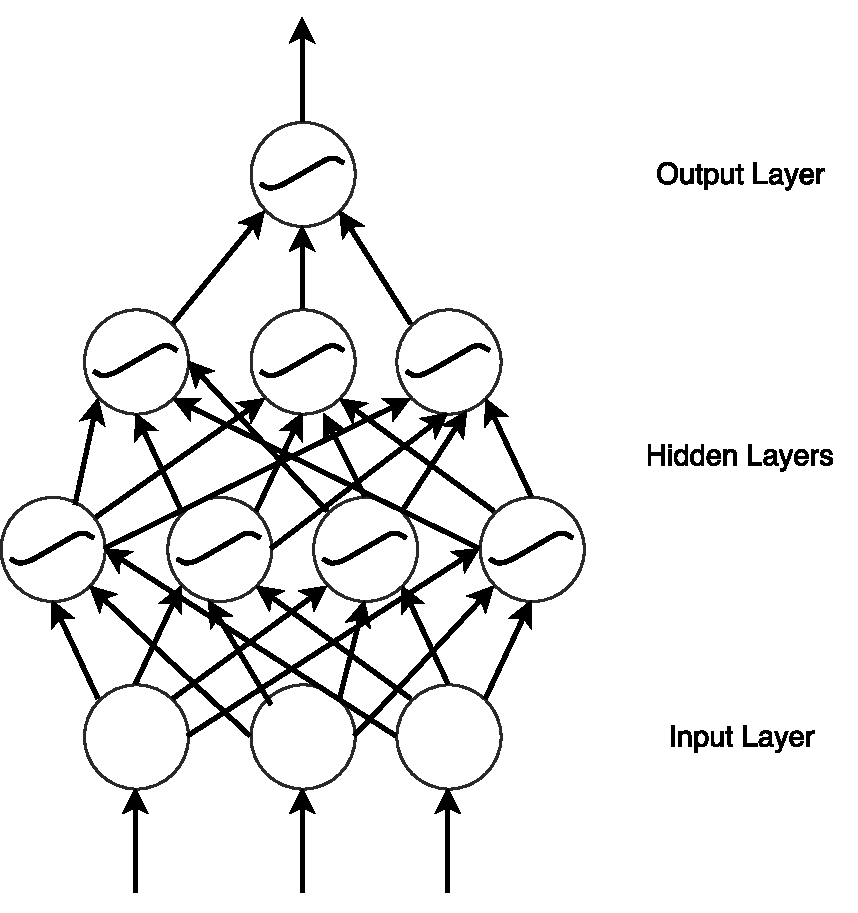
\includegraphics[width=\textwidth,height=\textheight,keepaspectratio]
    {Figures/mlp.pdf}
    \rule{35em}{0.5pt}
\caption{A feedforward neural netwrok with two hidden layers, this network is also known as a
multilayer perceptron. The S-shaped curves denote the sigmoidal function.}
\label{fig:ffnnetwork}
\end{figure}

\section{Deep recurrent networks}
As mentioned earlier, we can create a recurrent neural network by adding feedback connections to
a feedforward network. Several types of recurrent neural networks have been proposed over the
years, some of which are - \emph{echo state networks, time delay networks, jordan networks}. At
first the difference between a feedforward and a recurrent network may not be obvious and seem
trvial but recurrent networks are very powerful in the sense that they can retain the history and
thus forming a memory in their feedback connections.



\section{Network training}

\section{LSTM networks}
In previous section we learn that using a recurrent neural networks we can store information in
form of activations in the feedback connnections. The major disadvantage with recurrent neural
networks is their inability to ratain information for a long period of time. This is caused by an
effect known as \emph{vanishing gradient problem}(\citet{bengio1994learning},
\citet{hochreiter2001gradient}). The vanishing gradient problem is depicted in the figure
\ref{fig:vanishingGradient}. Number of attempts were made in the 1990's to resolve this issue.
\citet{hochreiter1997long} proposed a redesigned network called Long Short Term Momory(LSTM) to
address this problem.

\begin{figure}[htbp]
  \centering
    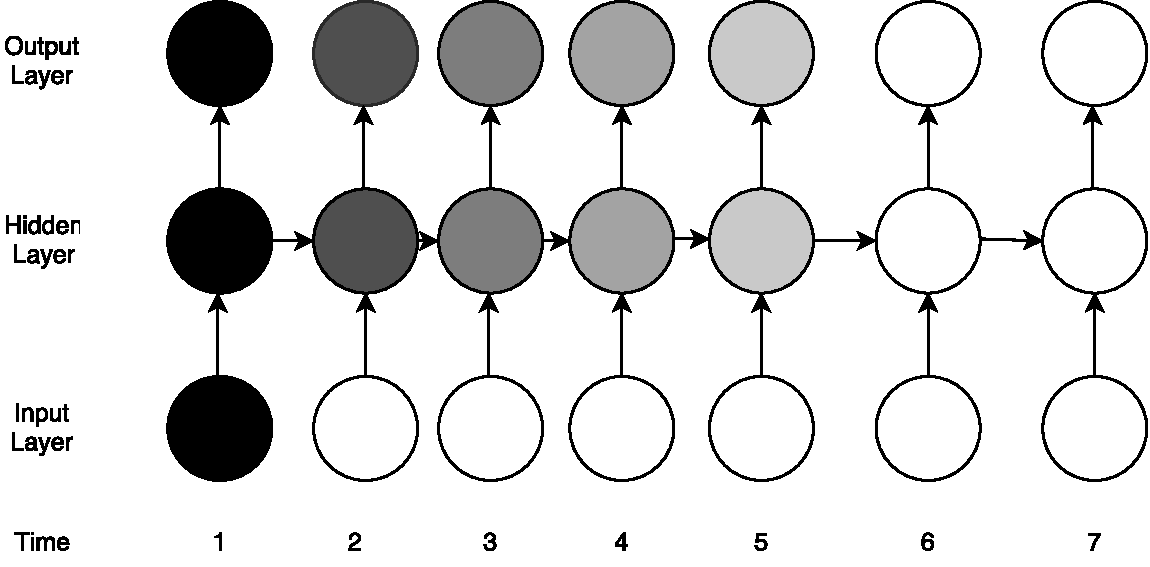
\includegraphics[width=\textwidth,height=\textheight,keepaspectratio]
    {Figures/vanishing-gradient.pdf}
    \rule{35em}{0.5pt}
  \caption[Vanishing Gradient] {The problem of vanishing gradient in recurrent neural networks.
  The sensitivity, as indicated by the shading, gradually diminishes with time}
  \label{fig:vanishingGradient}
\end{figure}


\subsection{Architecture}
An LSTM network is a set of recurrently connected LSTM blocks, also known as memory blocks, where
each memory block has one or more memory cells and three units (input, output and forget gates)
that perform the read, write and reset operations. The units allow the LSTM to store information
for a long time and thus addresses the problem of vanishing gradient. A basic LSTM block with one
memory cell is depicted in the figure \ref{fig:lstmBlock}

\begin{figure}[htbp]
  \centering
    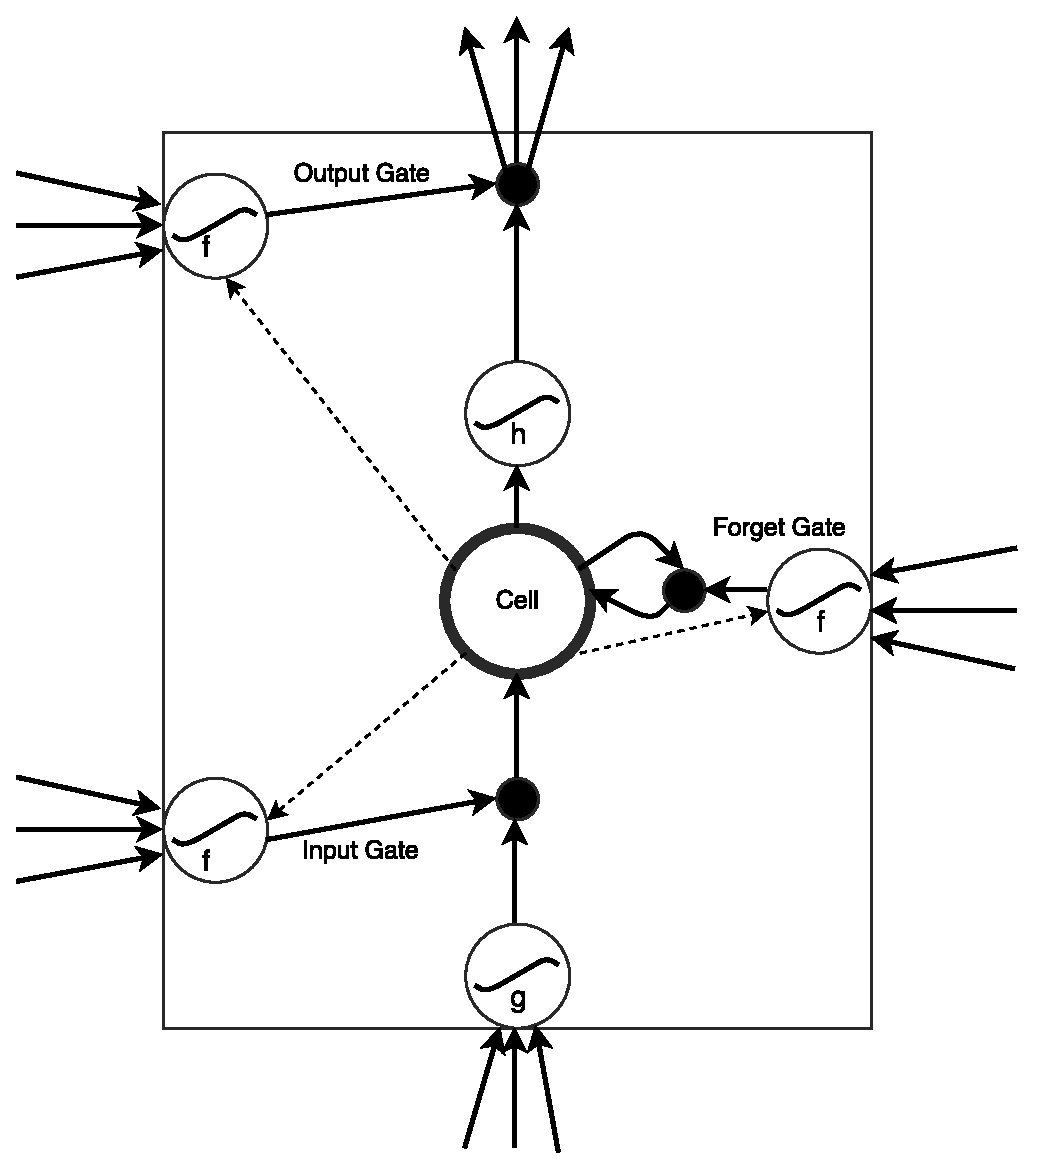
\includegraphics[width=\textwidth,height=\textheight,keepaspectratio]
    {Figures/lstm-block.pdf}
    \rule{35em}{0.5pt}
  \caption[An LSTM block with one cell]
{An LSTM block with one cell. The three units collect activations from both inside and outside of
the block. The small black circles represents mulitipications by which the gates control the
memory cell. The gate activation function is f, usually a logistic sigmoid. The cell input and
output functions are g and h, usually tanh or logistic sigmoid. The dashed lines represent the
weighted peephole connections from the cell to the gates. All other connections are not weighted.
The only outputs from the block to the rest of the network is from the output gate multiplication.}
  \label{fig:lstmBlock}
\end{figure}
% Chapter 5

\chapter{Experiments and Results} % Main chapter title

\label{Chapter5} % For referencing the chapter elsewhere, use \ref{Chapter5}

% This is for the header on each page - perhaps a shortened title
\lhead{Chapter 5. \emph{Experiments and Results}}

% Quotation
``Science, my boy, is made up of mistakes, but they are mistakes which it is useful to make,because
they lead little by little to the truth"

\begin{flushright}
Jules Verne, \textit{Journey to the Centre of the Earth} (1864)
\end{flushright}

%---------------------------------------------------------------------------------------------------
%	CONTENT
%---------------------------------------------------------------------------------------------------
%1892 VICTORIA STREET 12607 W BD 16911
%1893 VICTORIA STREET 12608 W BD 16912
%1897 VICTORIA STREET 12612 W BD 16913
% Hoddle st - 268 to 278 (South bound)
% Hoddle st - 10522 to 16517 (North bound)
% Bridge Road 14475 - 14479 (West bound)
% Barkers Road 16548 - 16551 (West bound)
% Princess st 6297 (South bound)
% Power st - 16537 - 16538 (North bound)

For our experiment we used various existing methods in short term traffic prediction along with the
deep neural network models. This is to perform a broad comparison among the methods. For
baseline model purpose we chose the naive method. For comparison purpose we chose Linear regression, ARIMA,
Exponential smoothing with state space model, Neural network autoregression with a single hidden layer, K nearest
neighbour and Support vector regression. We used three variants of deep recurrent networks - simple
RNN, Long Short Term Memory (LSTM) and Gated Recurrent Unit (GRU). For the purpose of our experiment we used the data, whose
details were presented in chapter \ref{Chapter3}. All the models used the data from the homogeneous road
section(HF No. 16913) on Victoria street between Hoddle street and Church street, as shown in the
figure \ref{fig:ExperimentRegion} annotated in red. We also used the data from neighbourhood locations
(the region annotated in blue) for training the deep neural networks to capture the spatial relationships.
For handling missing data, we used interpolation method. All the models were used for prediction
horizons of 15 minutes, 30 minutes and 45 minutes.


\section{Baselline and compared models}
In this section, we present the details of the experiments and results of the chosen baseline method
and the compared models. The naive method was used to set up a baseline, the naive method uses
the last observed value as the prediction. The results of the naive method is shown in
\ref{fig:baseline}. The plot shows that the naive method perform very well in predicting short
term traffic prediction. Also the main advantage is there is no significant computation is
required for calculating the prediction values.

\begin{figure}[htbp]
    \centering
    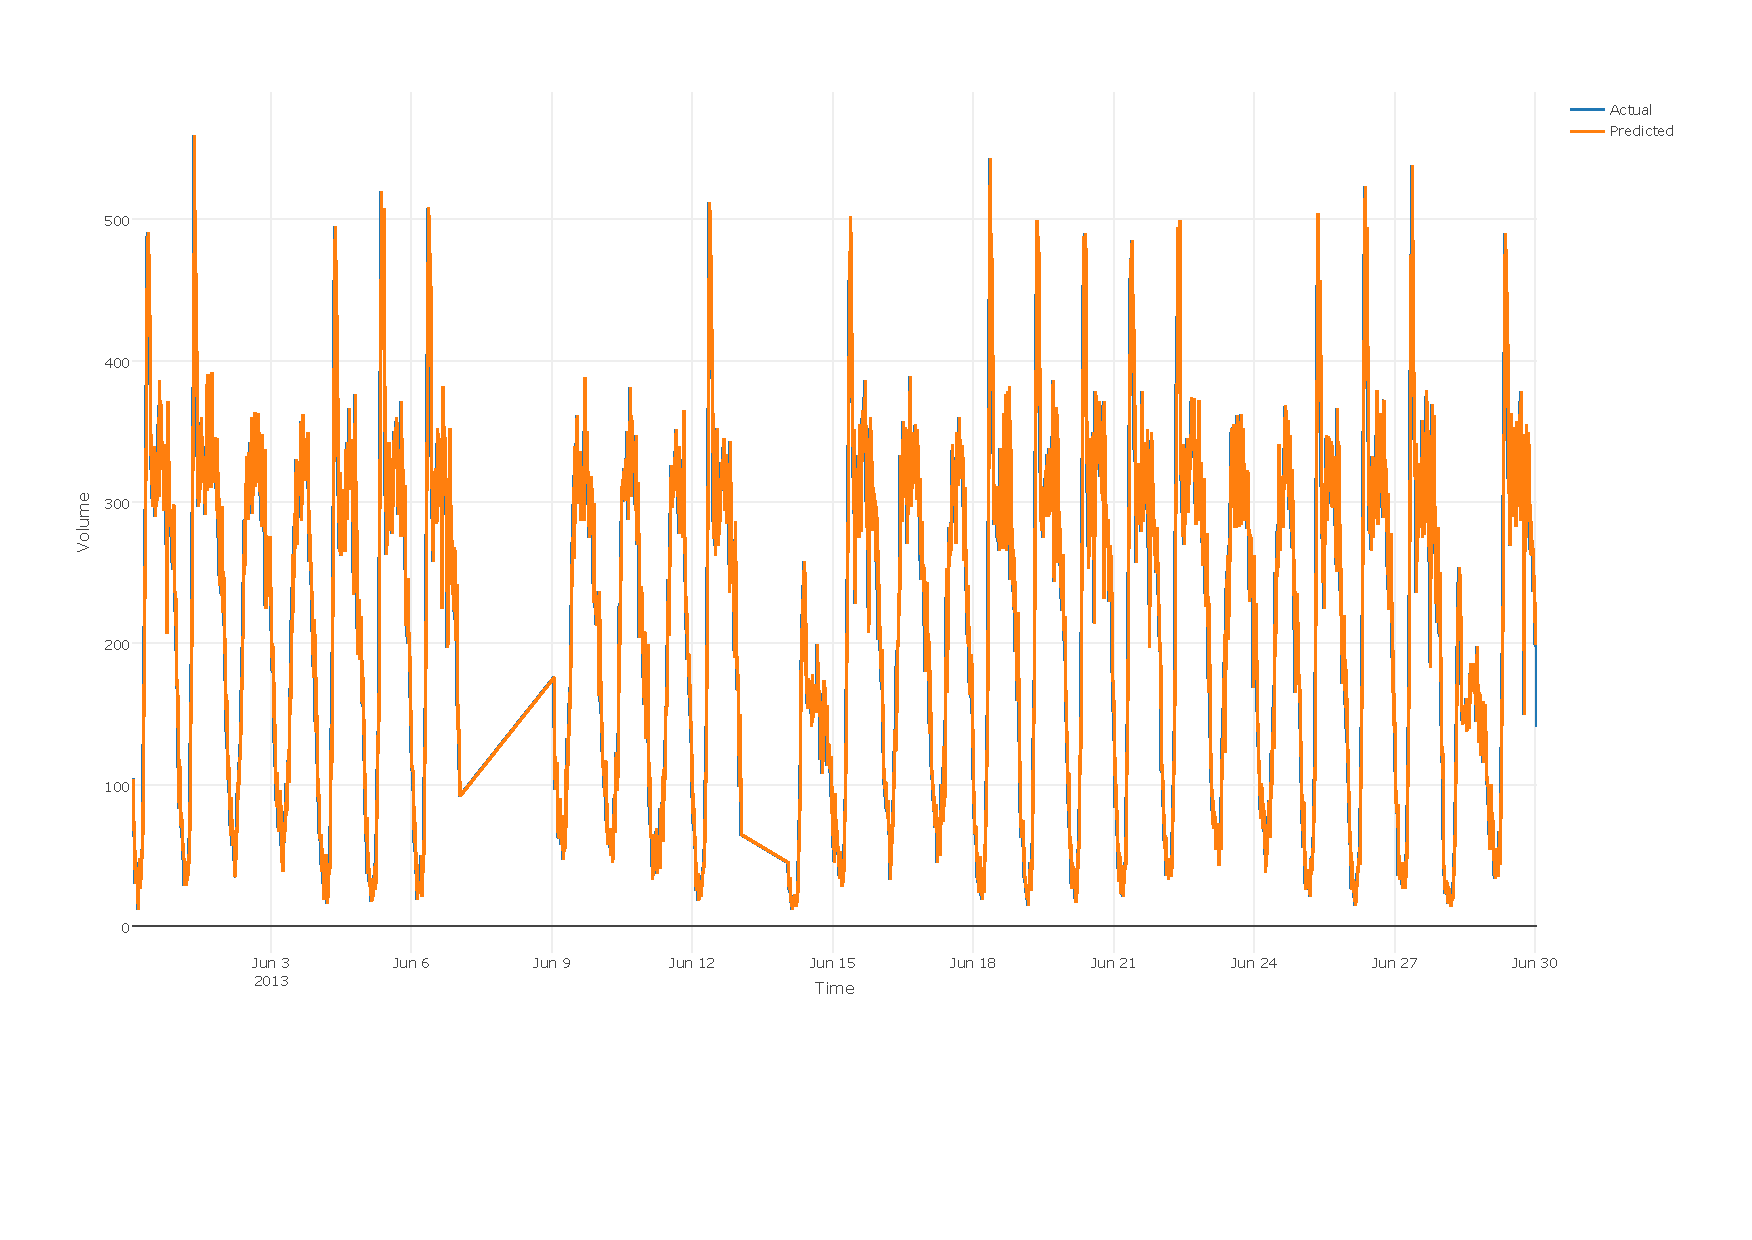
\includegraphics[width=0.7\textwidth]{Plots/naive1.pdf}
    \rule{35em}{0.5pt}
    \caption[Results of the Naive method]{Results of the Naive method, which is used as the baseline method.}
    \label{fig:baseline}
\end{figure}


Once the baseline is set, we used the comparing models to find out their performance. The results of
the comparing models are presented in figure \ref{fig:comparedModels}.

\begin{figure}[h]
    \centering
    \subfloat[Linear Regression][Linear Regression]{
    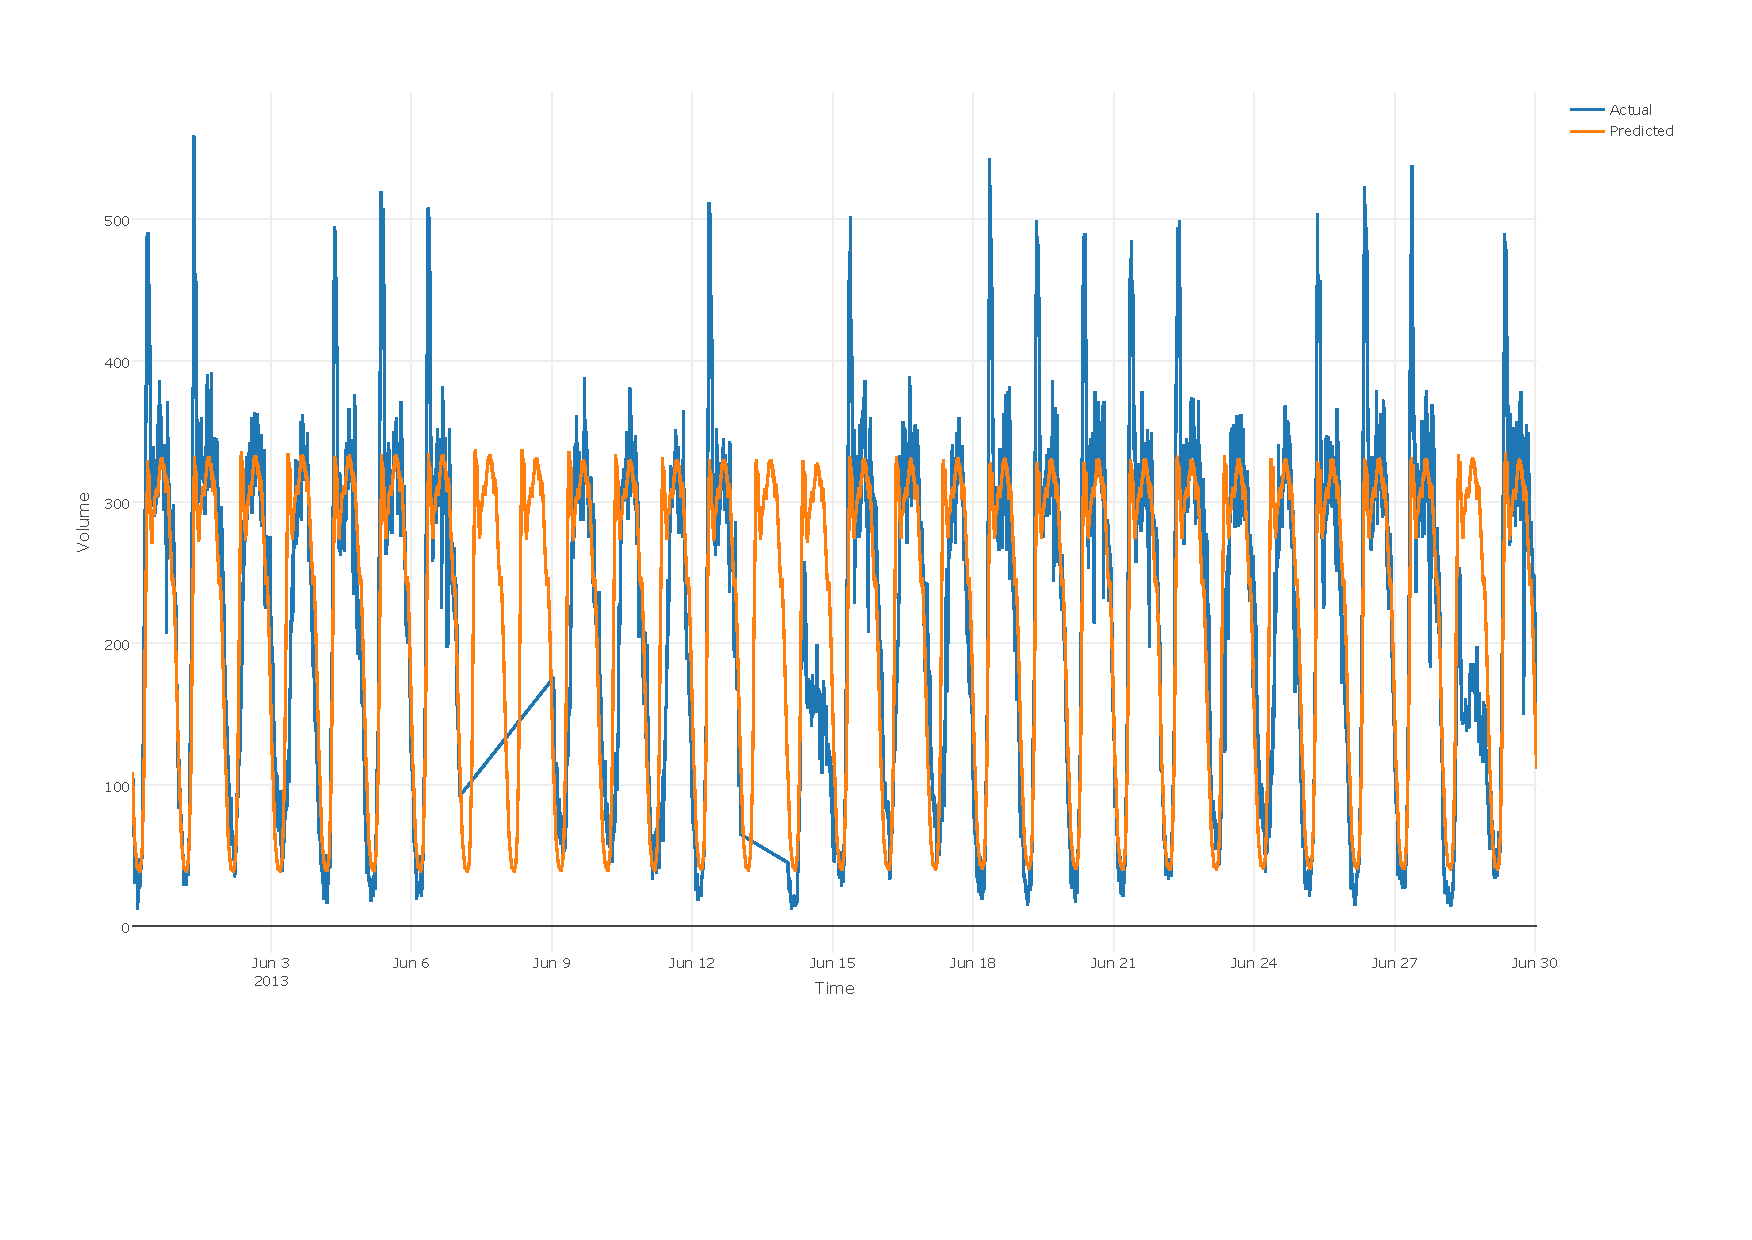
\includegraphics[width=0.4\textwidth]{Plots/linear1.pdf}
    \label{fig:lm1ActualPredicted}}
    \qquad
    \subfloat[ARIMA][ARIMA]{
    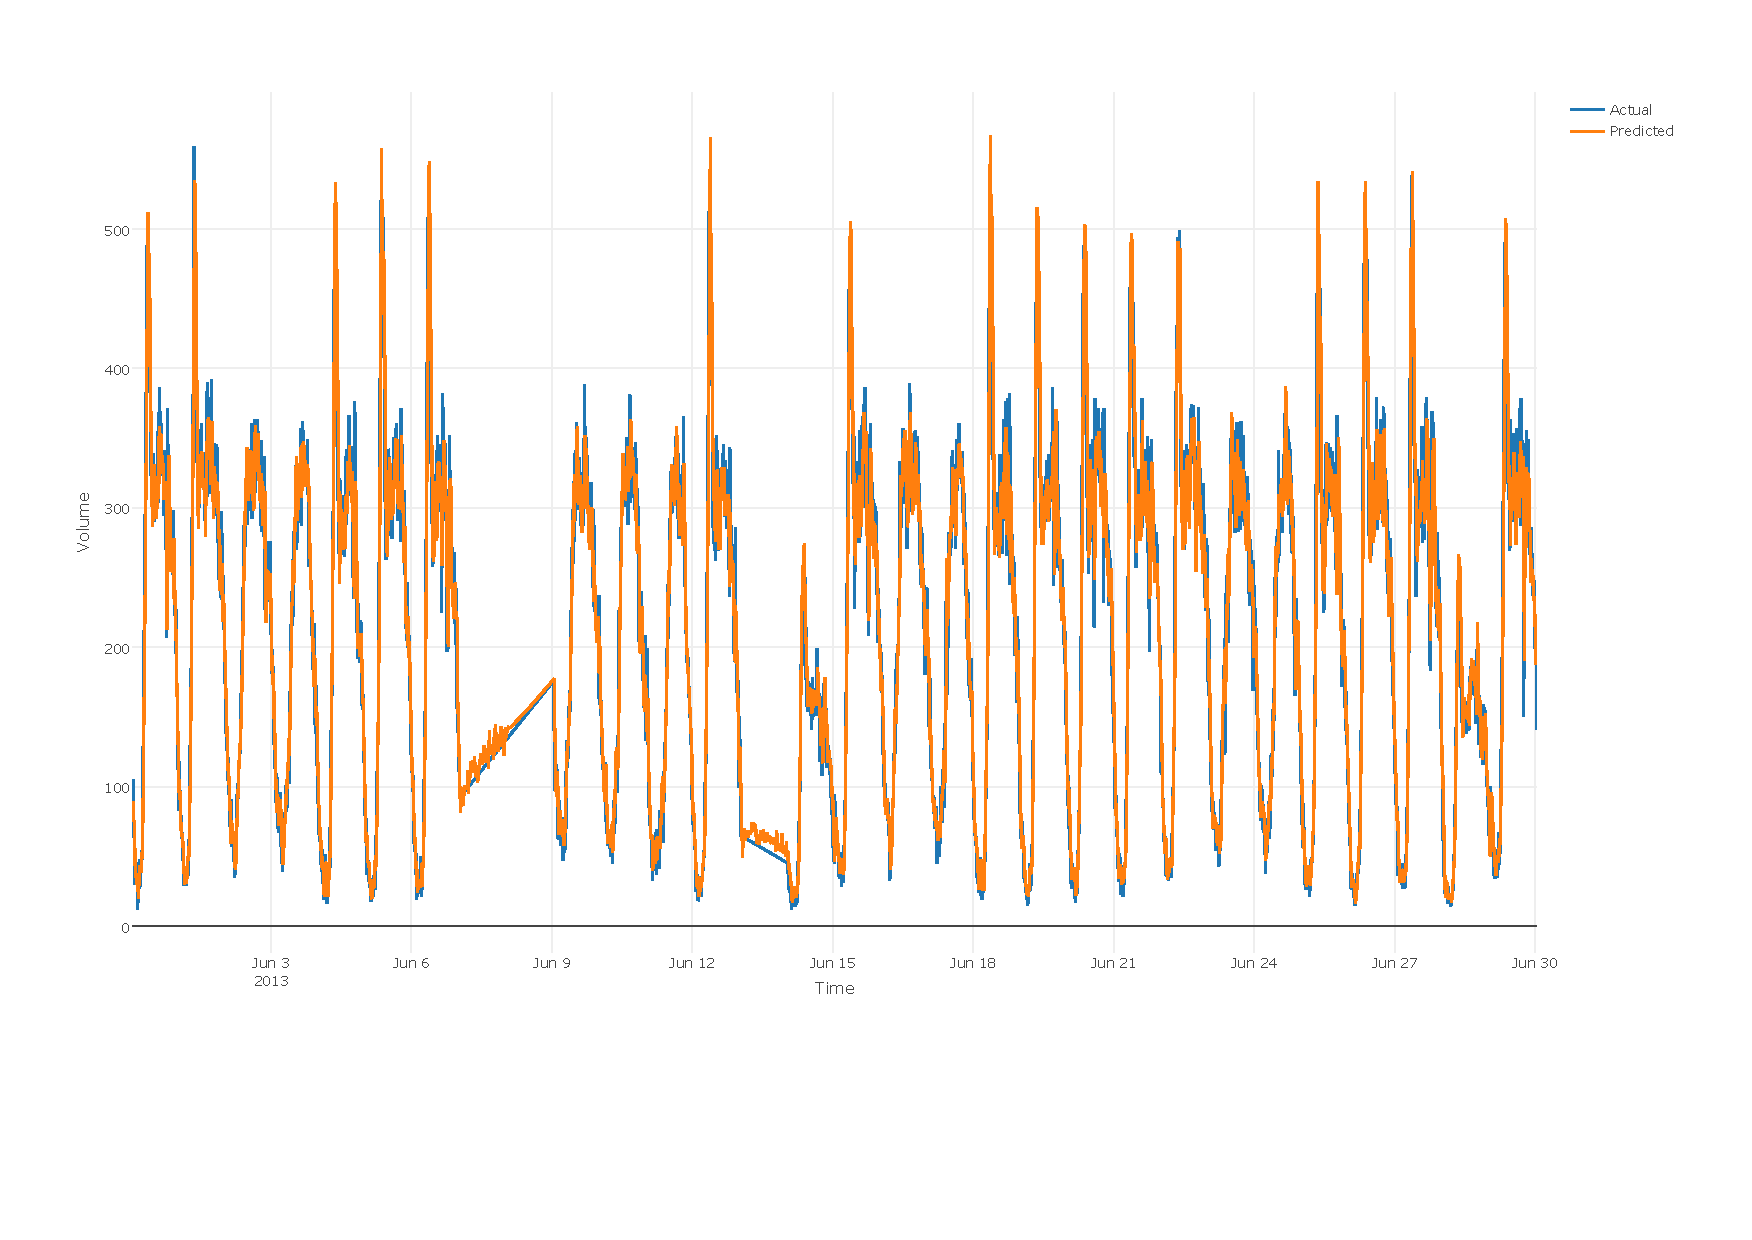
\includegraphics[width=0.4\textwidth]{Plots/arima1.pdf}
    \label{fig:arima1ActualPredicted}}

    \subfloat[Exponential smoothing state space model][Exponential smoothing state space model]{
    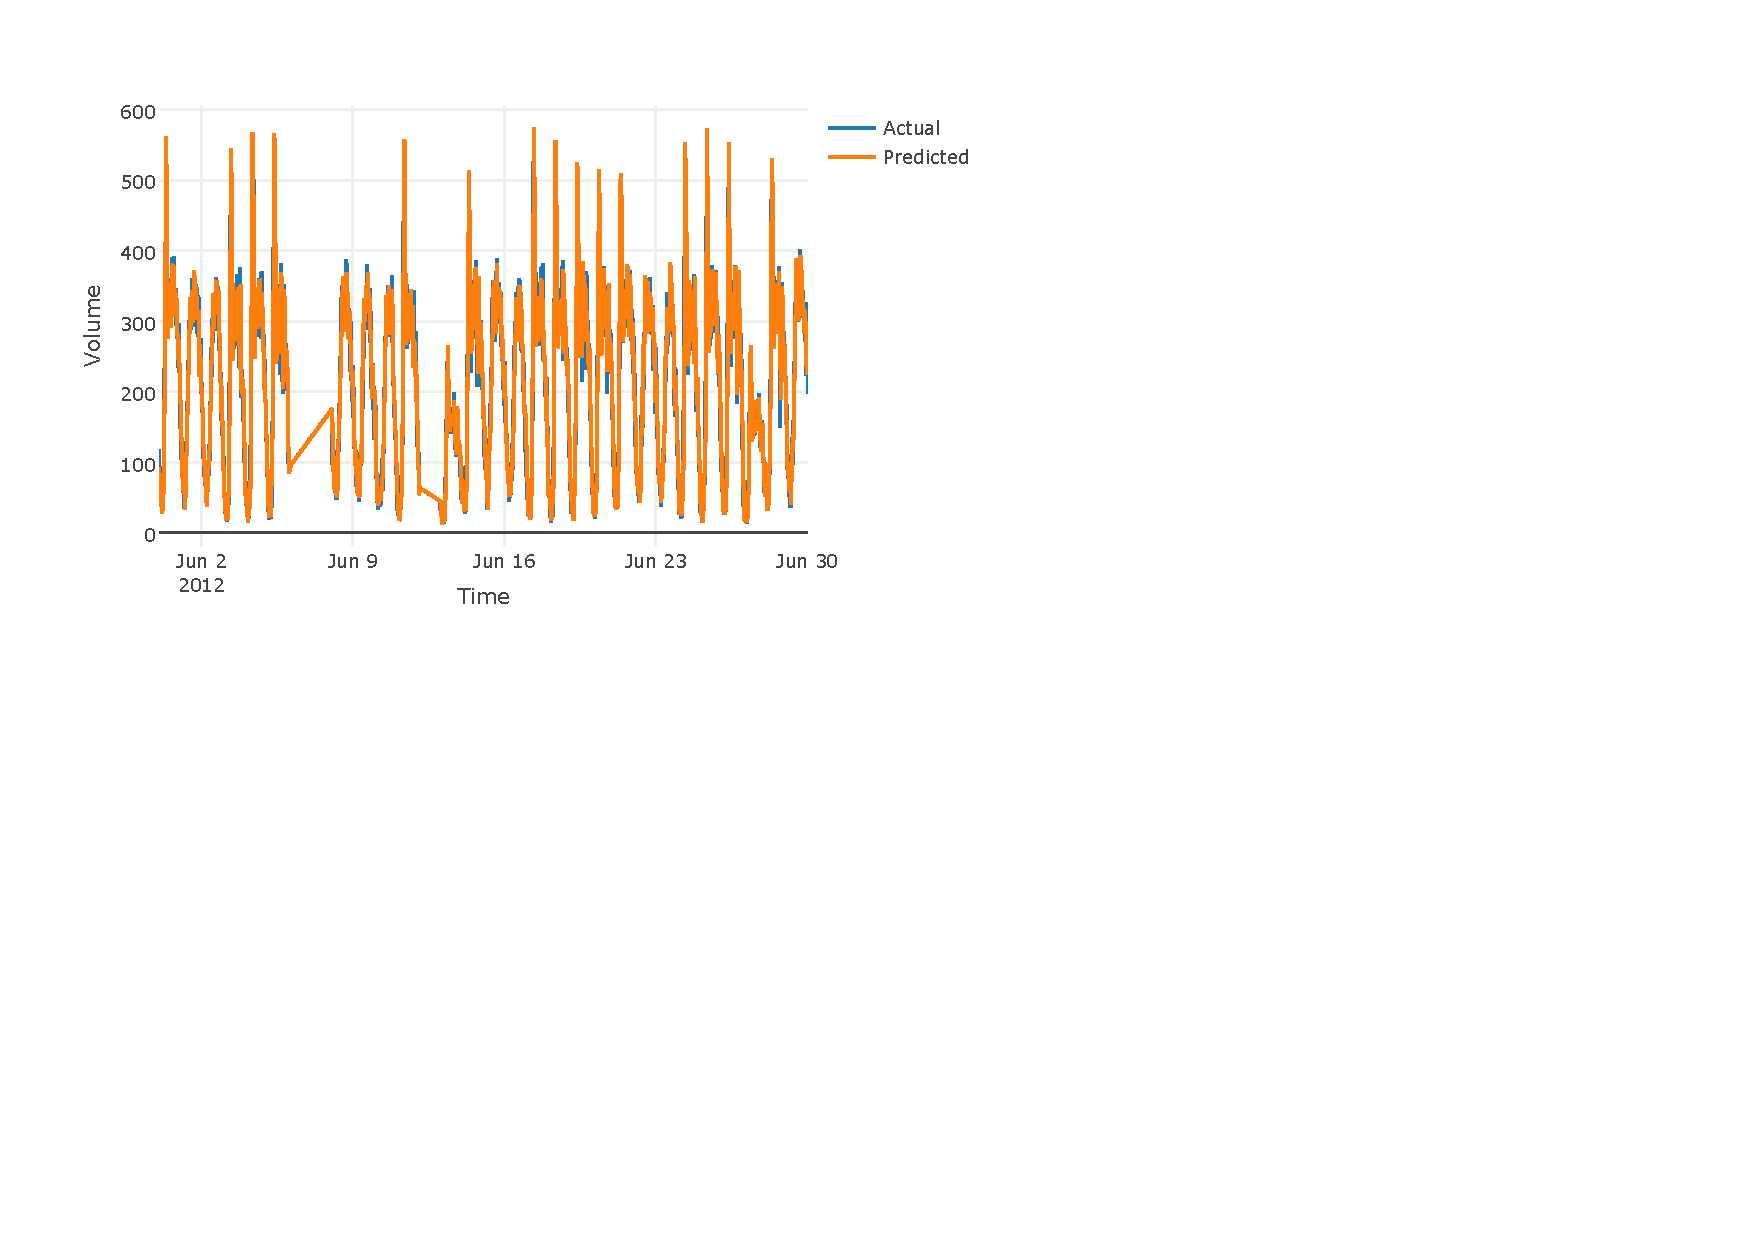
\includegraphics[width=0.4\textwidth]{Plots/ets1.pdf}
    \label{fig:ets1ActualPredicted}}
    \qquad
    \subfloat[Neural Network AutoRegression][Neural Network AutoRegression]{
    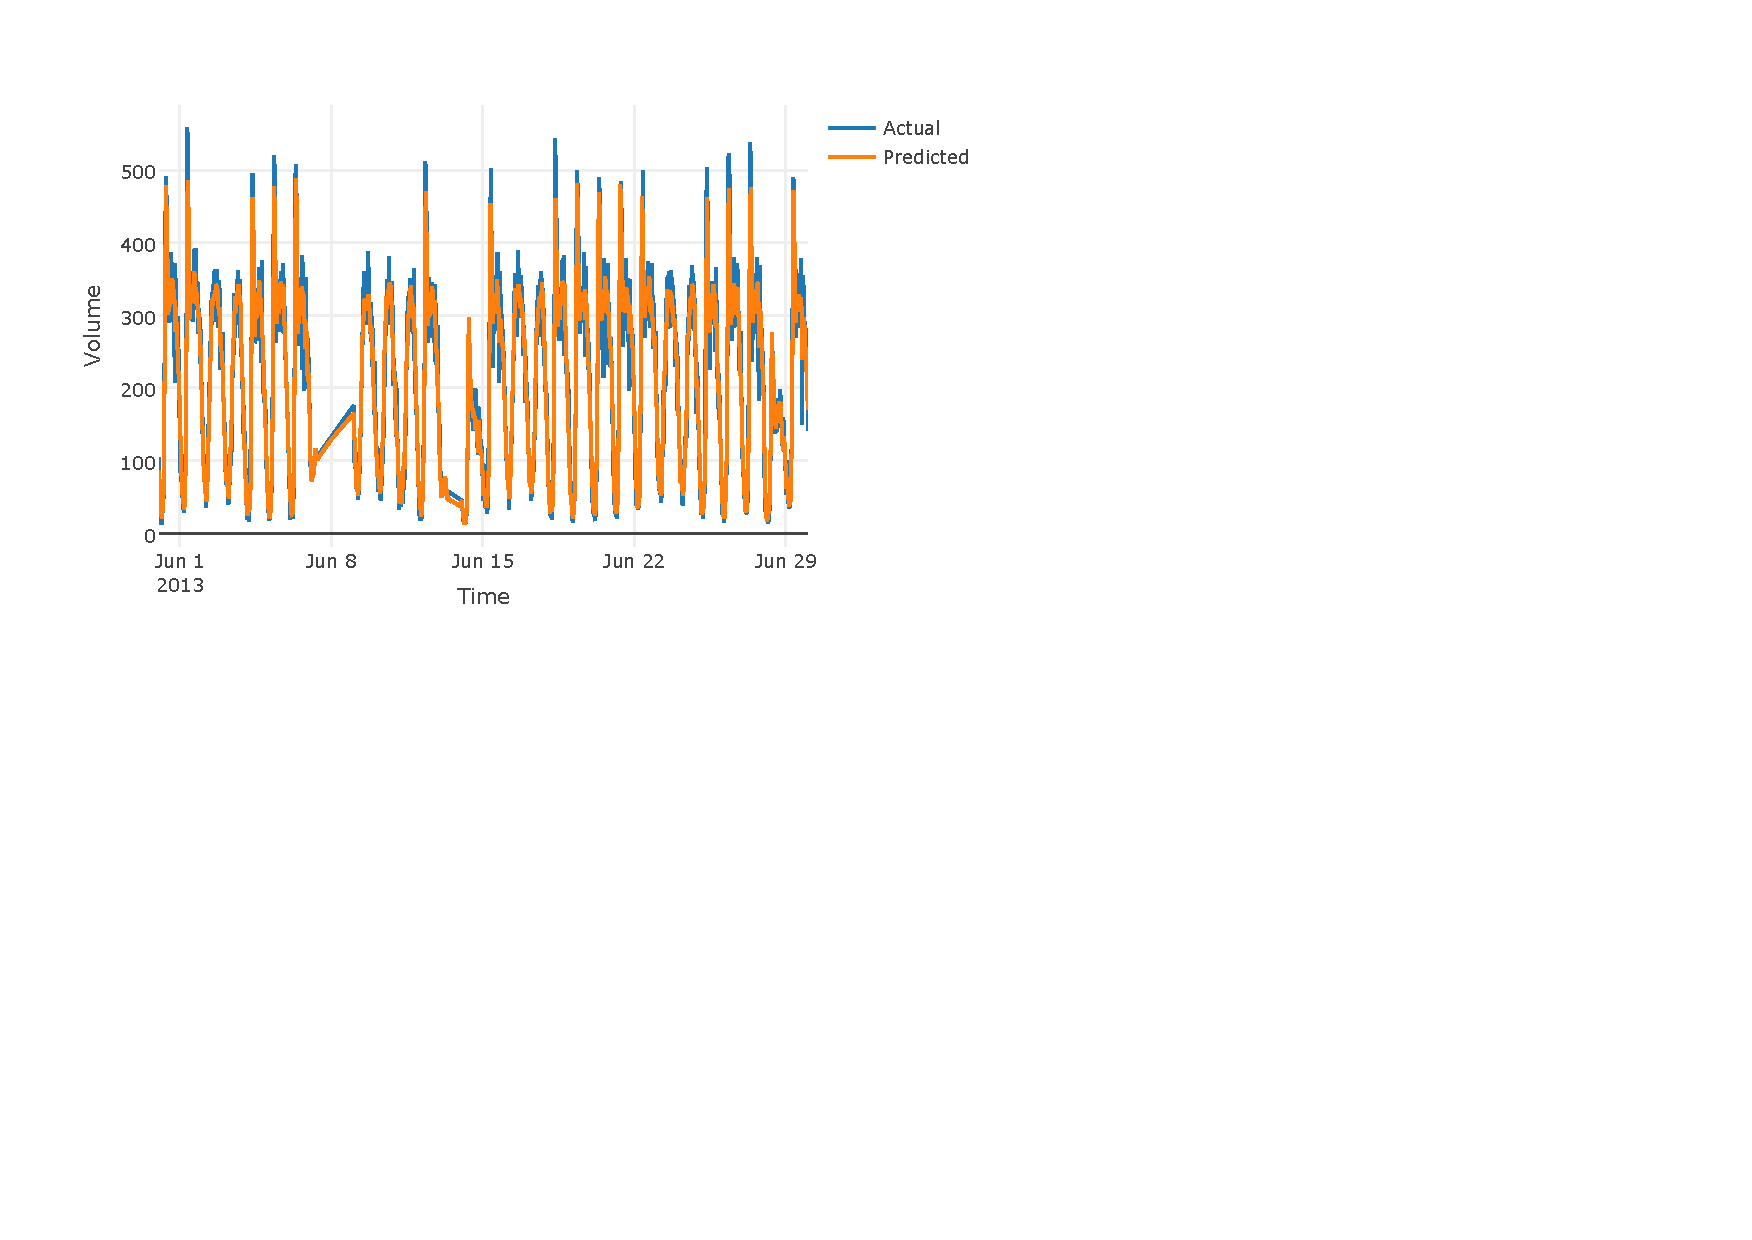
\includegraphics[width=0.4\textwidth]{Plots/nnetar1.pdf}
    \label{fig:nnetar1ActualPredicted}}

    \subfloat[K-Nearest Neighbour][K-Nearest Neighbour]{
    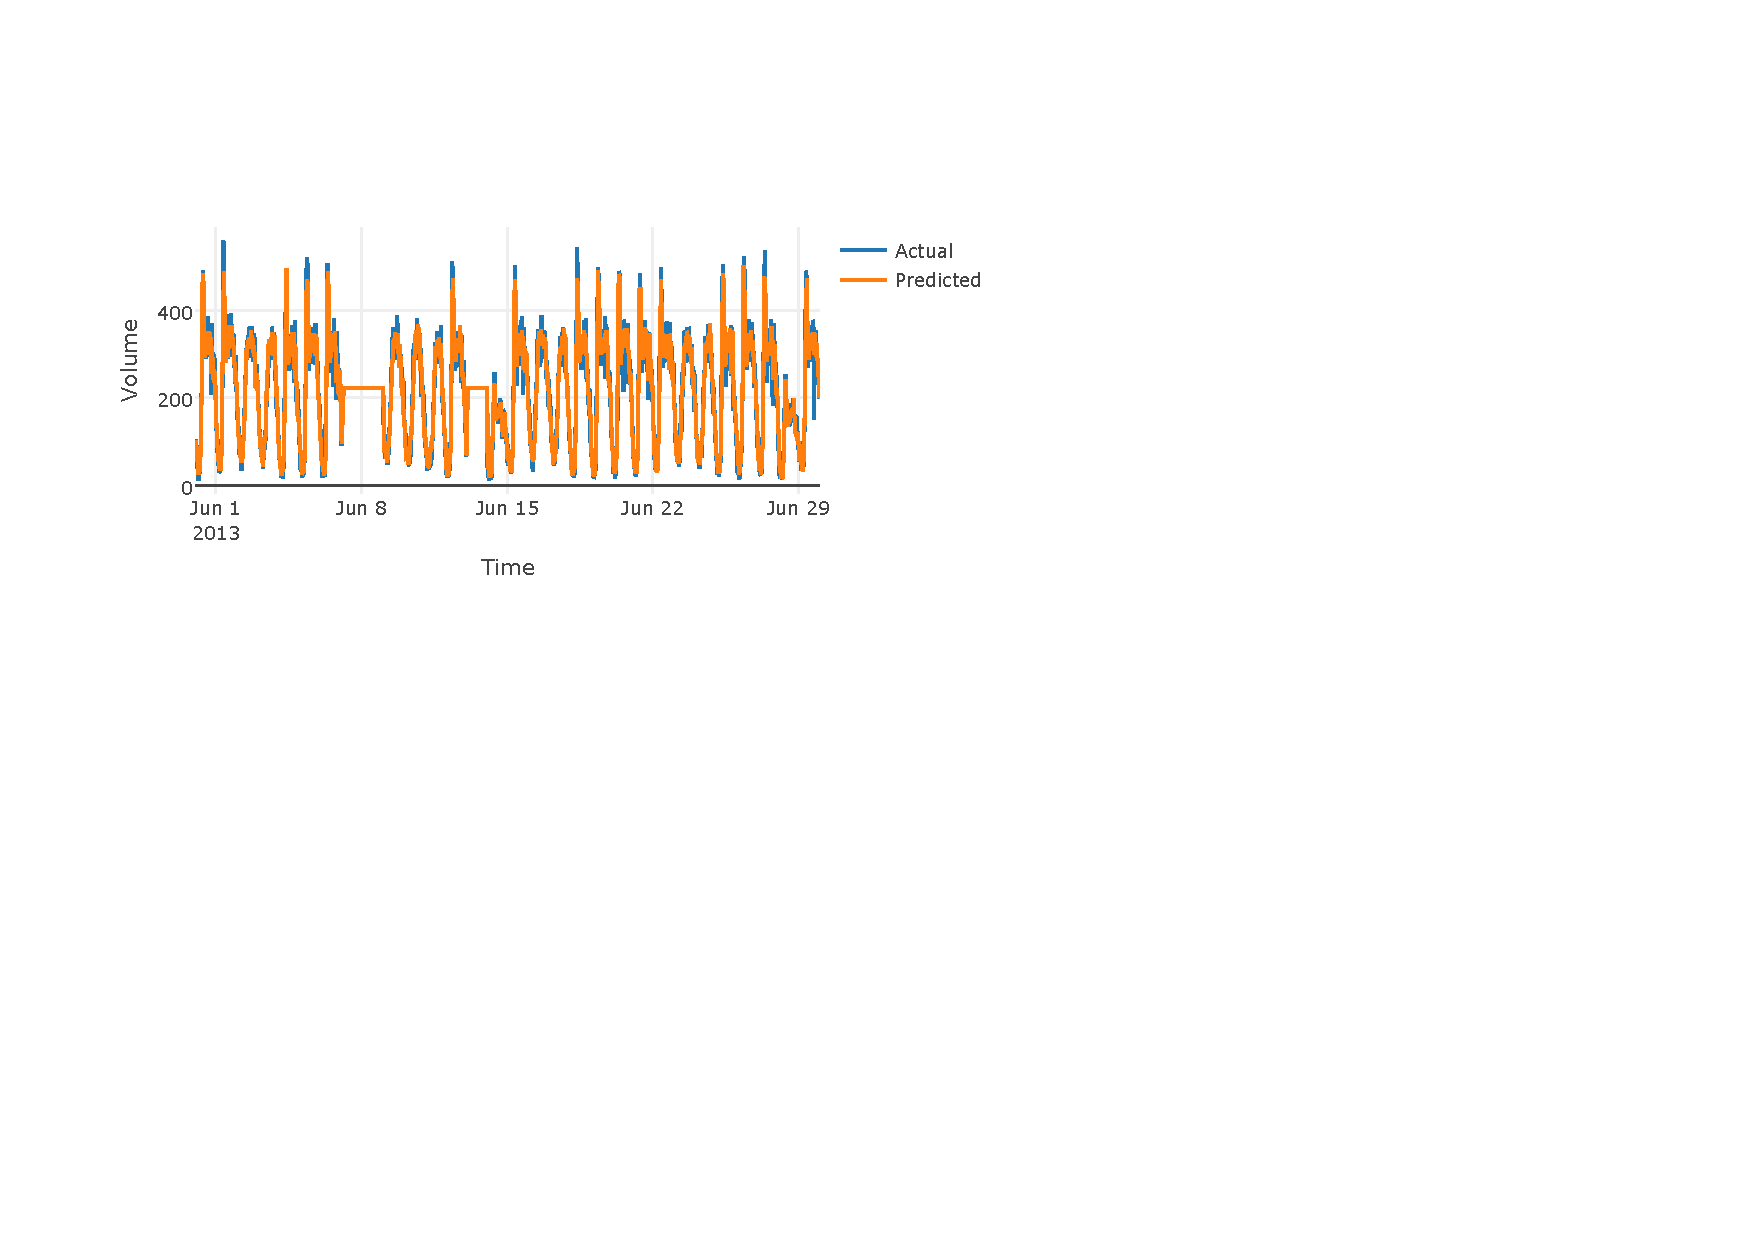
\includegraphics[width=0.4\textwidth]{Plots/knn1.pdf}
    \label{fig:knn1ActualPredicted}}
    \qquad
    \subfloat[Support Vector Regression][Support Vector Regression]{
    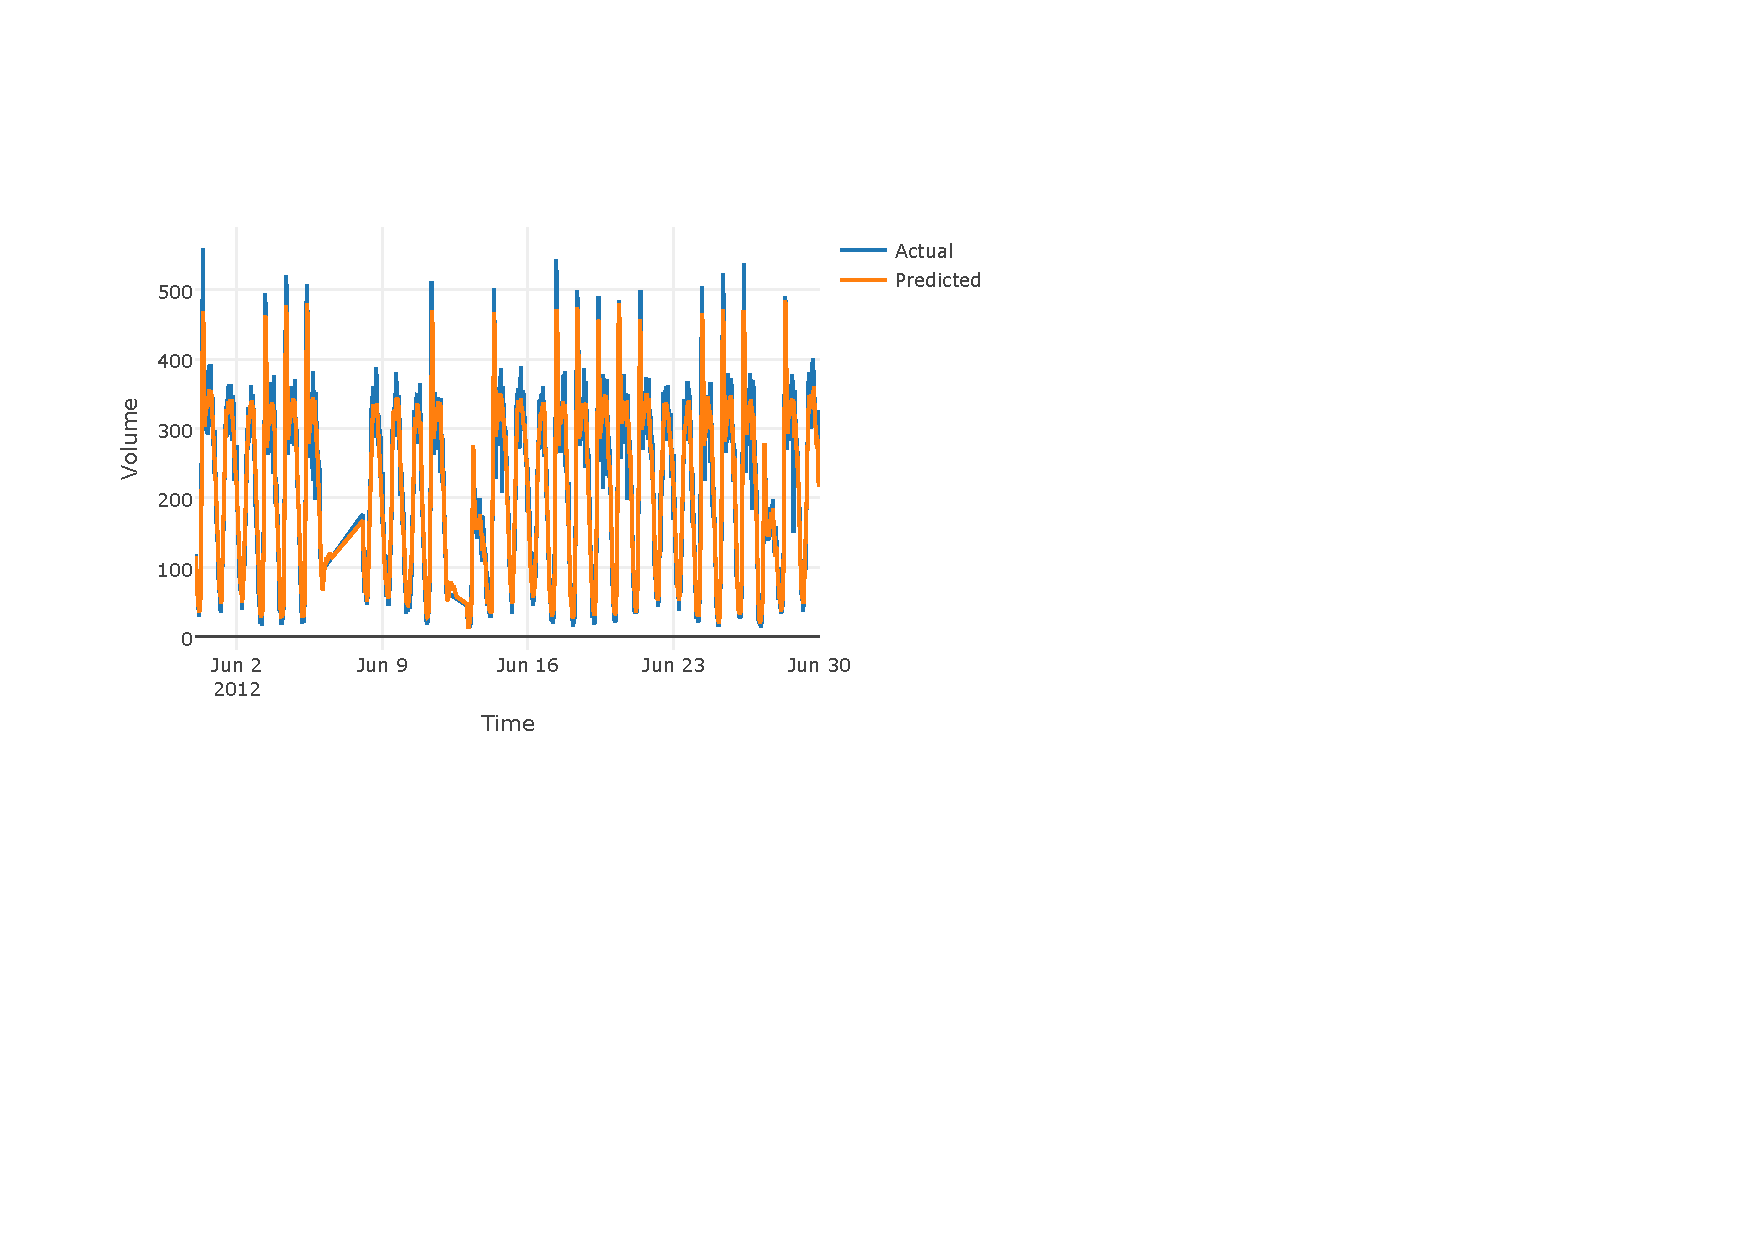
\includegraphics[width=0.4\textwidth]{Plots/svm1.pdf}
    \label{fig:svm1ActualPredicted}}

    \caption[Actual vs Predictions, using currently popular methods]{Actual vs Predictions -
    naive, linear regression, ARIMA, simple feed forward neural network with one hidden layer, exponential
    smoothing using state space model, k-nearest neighbour and support vector regression.
    The models were trained on traffic data from one homogeneous road segment. The plots show the
    actual vs predictions (15 mins) for the month of June 2012.}
    \label{fig:comparedModels}
\end{figure}


\begin{itemize}

\item \textbf{Linear regression}: We used a linear model for time series regression. The model was
created using the season component of the traffic volume time series data. The model
did not perform well, in fact its performance was the worst among all the models used in this
experiment.

\item \textbf{ARIMA}: After handling missing data, the Box-Cox transformation was done to stabilise the
variance. Then Using the Hyndman-Khandakar algorithm, the best ARIMA model was chosen. The selected
model was a seasonal ARIMA(2,0,5)(1,0,0)[96]. The model was fit using data from January to May 2012 with
frequency 96. Once the model was fit forecasts at steps 1 to 3 (15,30 and 45 minutes horizon) were
done in a recursive manner, that is after every forecast the model was refit using the newly available
observed data. The ARIMA model performed better than the baseline.

\item \textbf{Exponential smoothing}: For exponential smoothing, a state space model was used. This
model was a damped linear method with additive errors. Data preprocessing was done by handling missing
data through interpolation and then applying Box-Cox transformation to stabilise the variance. The
model used the same data used for the ARIMA model. The performance of the model was worse when compared
to the ARIMA model.

\item \textbf{Neural network autoregression}: A simple feedforward network with one hidden layer
was used. The lagged values of traffic volume time series were used as inputs to this network. A
38-20-1 neural network with 801 weights was used. Again for training purpose the same data that
was used for ARIMA and exponential smoothing methods were used. The performance of this model
was very good, better than the ARIMA model.

\item \textbf{K Nearest neighbour}: A neighbour based regression model was used, where the number
of nearest neighbours, k is set to 5. This value was selected by using both the autocorrelations and
cross validations. The distance measure was used to assign weights to each value in the local
neighbourhood.

\item \textbf{Support vector regression}: An epsilon-SVR with RBF kernel was used for this experiment.
The input data was standardised to mean 0 and variance 1.

\end{itemize}

\section{Deep neural network models}
The experiment details of the three used models are presented below.
We used these models on two sets of data. First dataset is from a single location as mentioned earlier.
The second dataset consisted of the traffic volume data from the location of interest along with data
from 10 other locations in the neighbourhood.
The input data used were standardised to mean zero and variance 1. We used various setting for
length of the sequence, number of hidden layers and number of units in those layers and optimisation
algorithms used for optimising the gradients. We present the final settings of these models below.
The results of these models are shown in the figure \ref{fig:deepNNModels}.

\begin{itemize}

\item \textbf{Simple RNN}: The simple RNN used was a fully connected RNN where the output was fed
back to the input is used. For univariate modelling, that is using data from a single location and
make predictions for that location, the RNN model with 2 hidden layers with 100 units in each
layer was used. To avoid overfitting a dropout of 10\% was used at both the hidden layers. The weights
were initialised randomly using the uniform distribution. A linear activation function was used
in the output layer. The loss function used for training was the mean squared error. Finally for
optimising gradients, the RMSprop algorithm, which was proposed by Geoff Hinton, was used.
The RMSprop is an adaptive learning rate algorithm. The input data was a set of sequences, where
each sequence was created with 50 time steps. We trained the model for 30 epochs.
For multivariate modelling three hidden layers with number of units [100,200,200] were used.
The weight initialisations, optimising algorithm and error functions were same as the univariate model.

\item \textbf{GRU}: Gated Recurrent Unit is a simple version of LSTM and was recently proposed.
Similar to the simple RNN modelling, we used GRU to model both univariate and multivariate datasets.
For univariate model, the network consisted of two hidden layers with 100 units in each of them.
We used the RMSprop algorithm for gradient optimisation. The number of epochs used was 30. Similar to
the RNN network input data was a set of sequences, where each sequence was created with 50 time steps.
For multivariate modelling we used three hidden layers with number of units [100,200,200].

\item \textbf{LSTM}: An LSTM model was also implemented for modelling both univariate and multivariate
traffic volume datasets, similar to the above RNN and GRU networks. For univariate modelling number
of combinations of hidden layers and units in those were used. The final univariate model consisted
of two hidden layers with 100 and 200 units in them. The output layer had an linear activation function.
Different sequence lengths were used and a final length of 50 was selected. For optimisation purpose
we tried both the RMSprop and Adaptive Moment Estimation (ADAM) algorithms. We found that the
ADAM algorithm outperformed the RMSprop. We trained the network for 20 epochs. For multivariate
modelling we used three hidden layer with [100,200,200] units. Again we compared the RMSprop and ADAM
optimisation algorithms and found the later outperformed the former again.

\end{itemize}


\begin{figure}[h]
    \centering

    \subfloat[LSTM - single location][LSTM - single location]{
    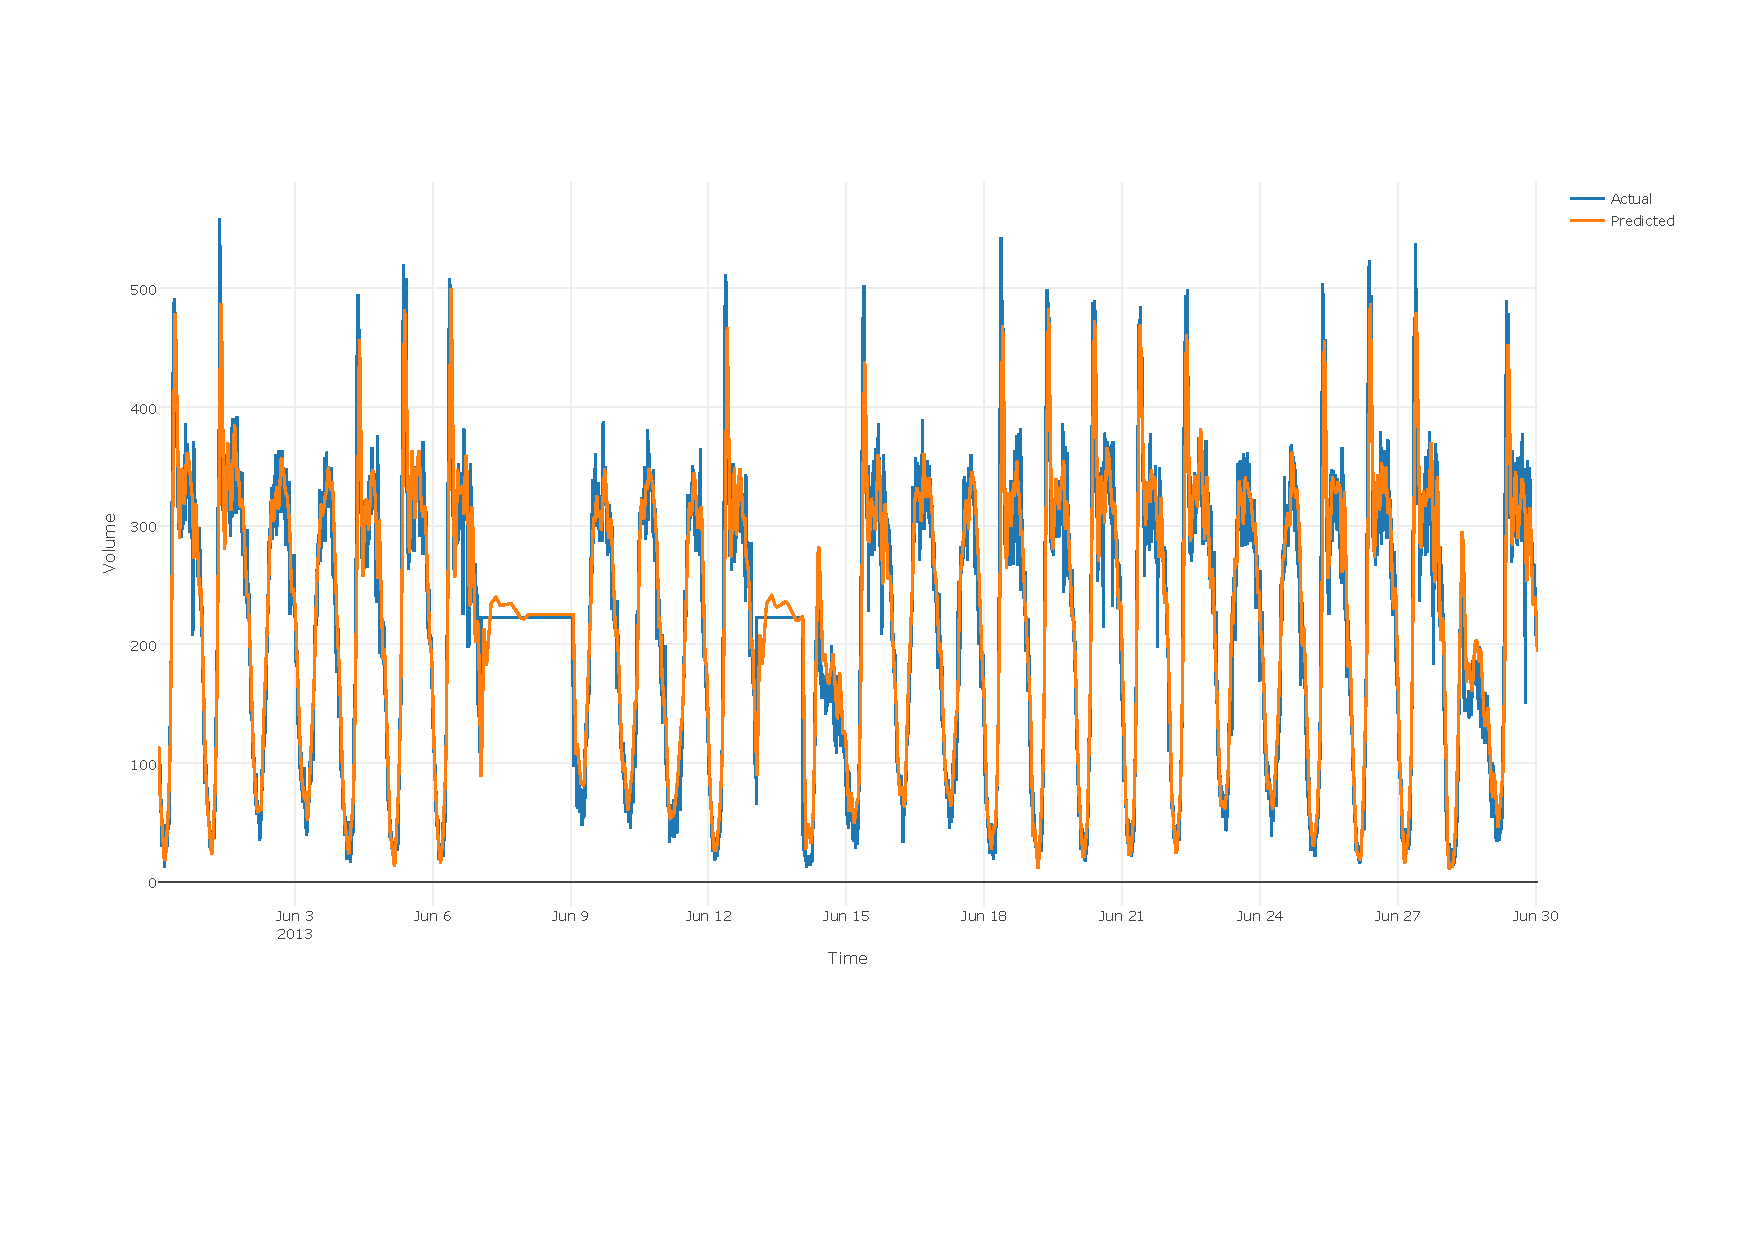
\includegraphics[width=0.4\textwidth]{Plots/lstm-single1.pdf}
    \label{fig:LSTMActualPredicted1}}
    \qquad
    \subfloat[GRU - single location][GRU - single location]{
    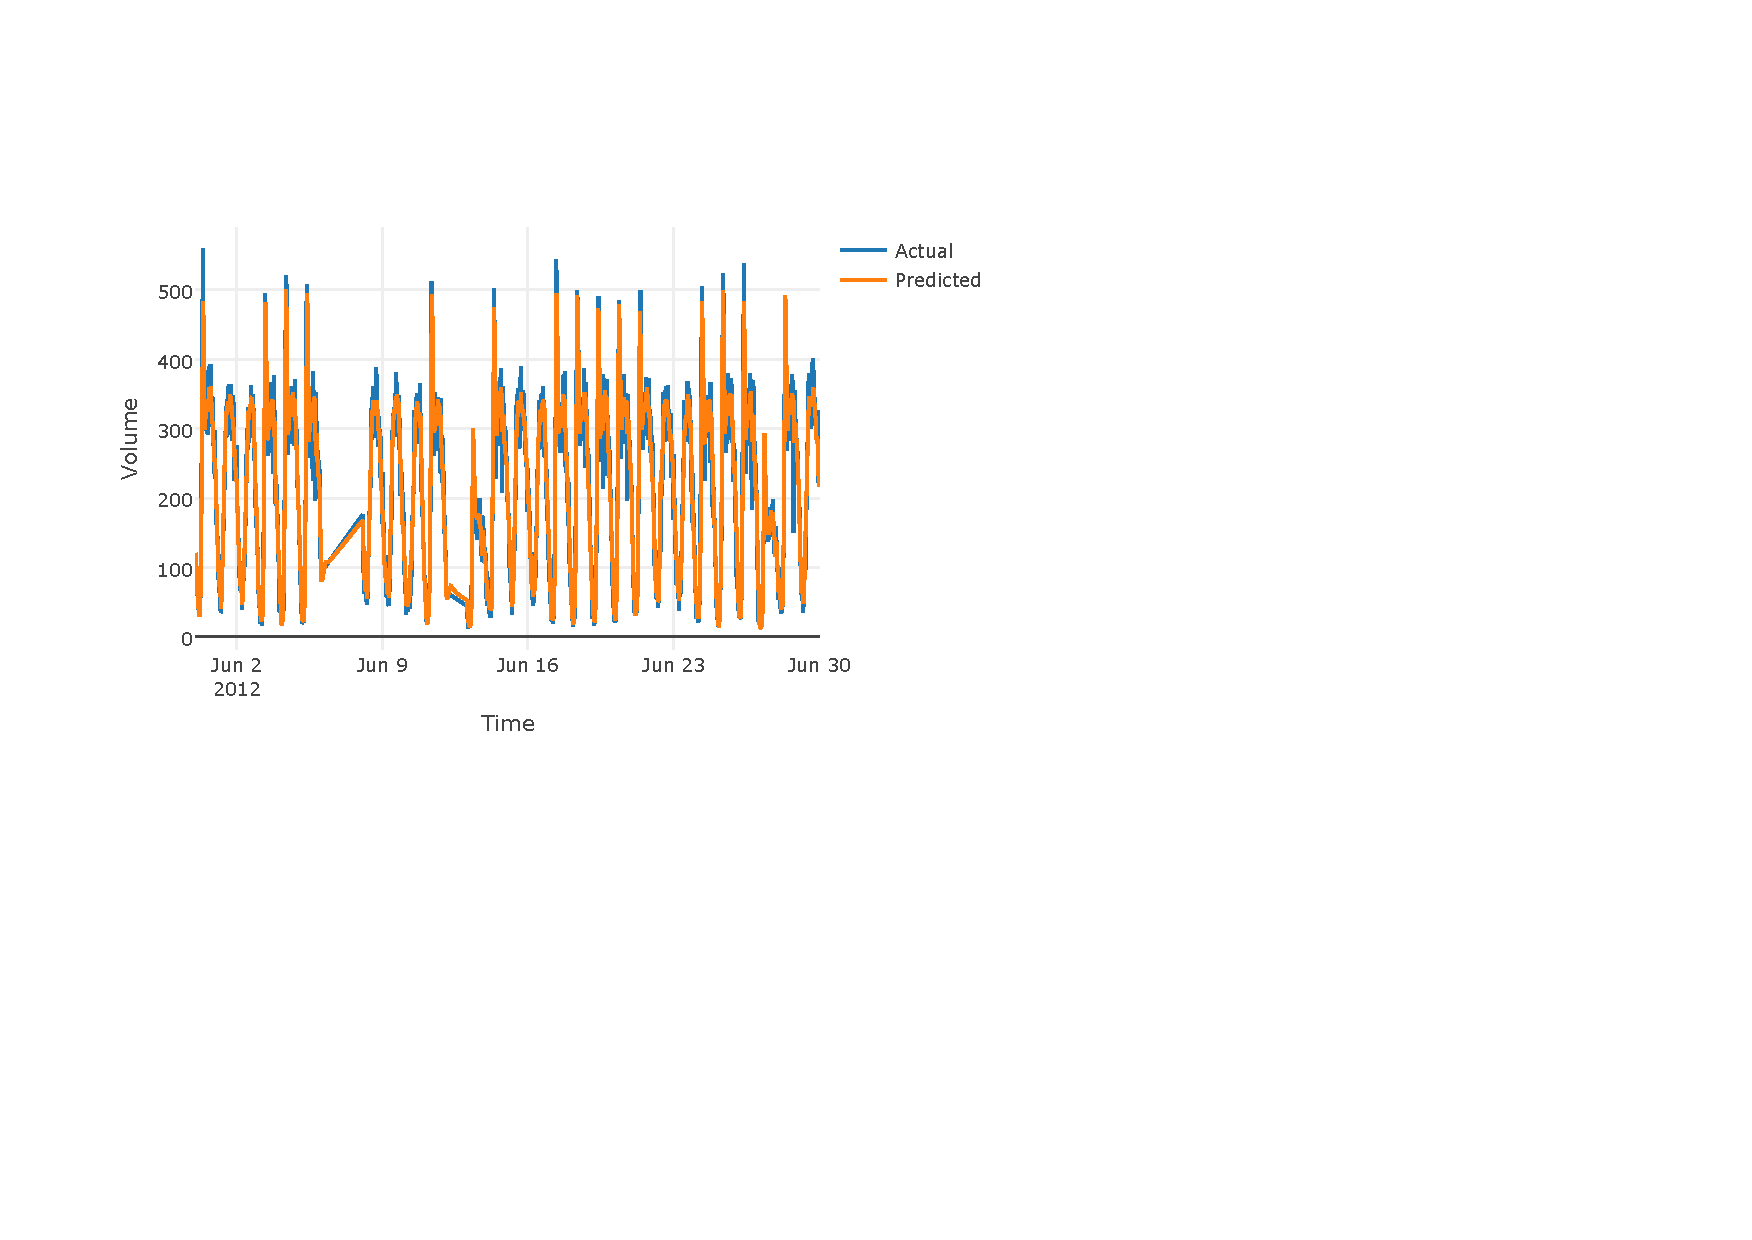
\includegraphics[width=0.4\textwidth]{Plots/gru-single1.pdf}
    \label{fig:GRUActualPredicted1}}

    \subfloat[RNN - single location][RNN - single location]{
    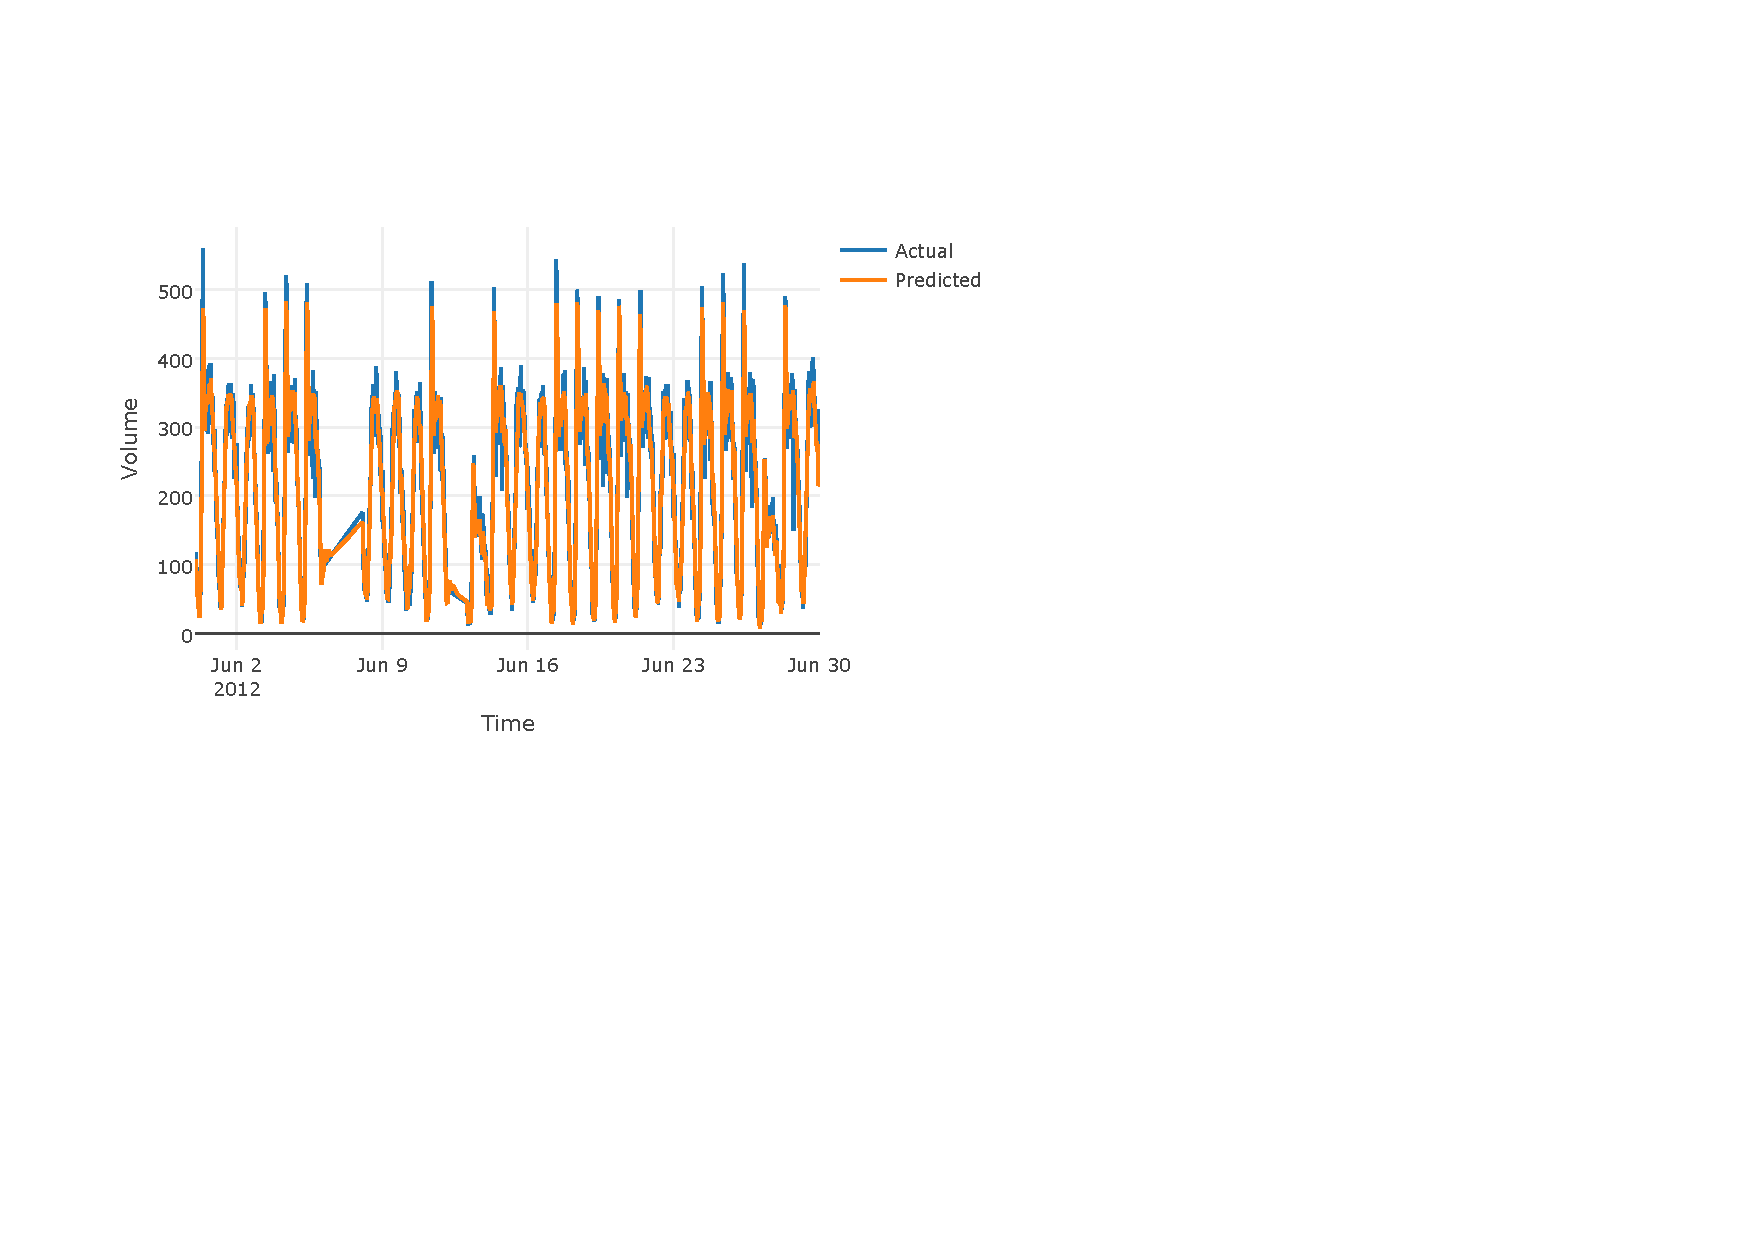
\includegraphics[width=0.4\textwidth]{Plots/rnn-single1.pdf}
    \label{fig:RNNActualPredicted1}}
    \qquad
    \subfloat[LSTM - multiple locations][LSTM - multiple locations]{
    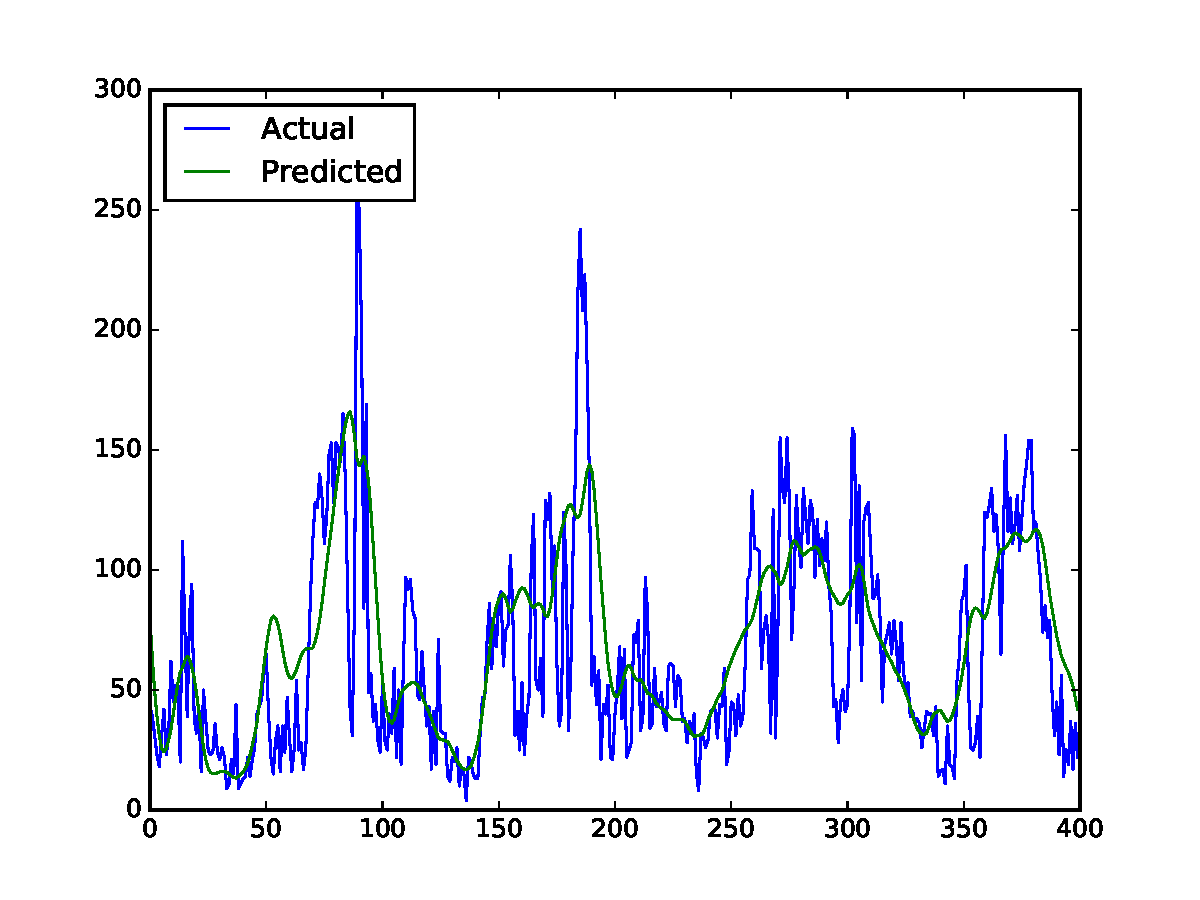
\includegraphics[width=0.4\textwidth]{Plots/lstm-multi1.pdf}
    \label{fig:LSTMMultiActualPredicted1}}

    \subfloat[GRU - multiple locations][GRU - multiple locations]{
    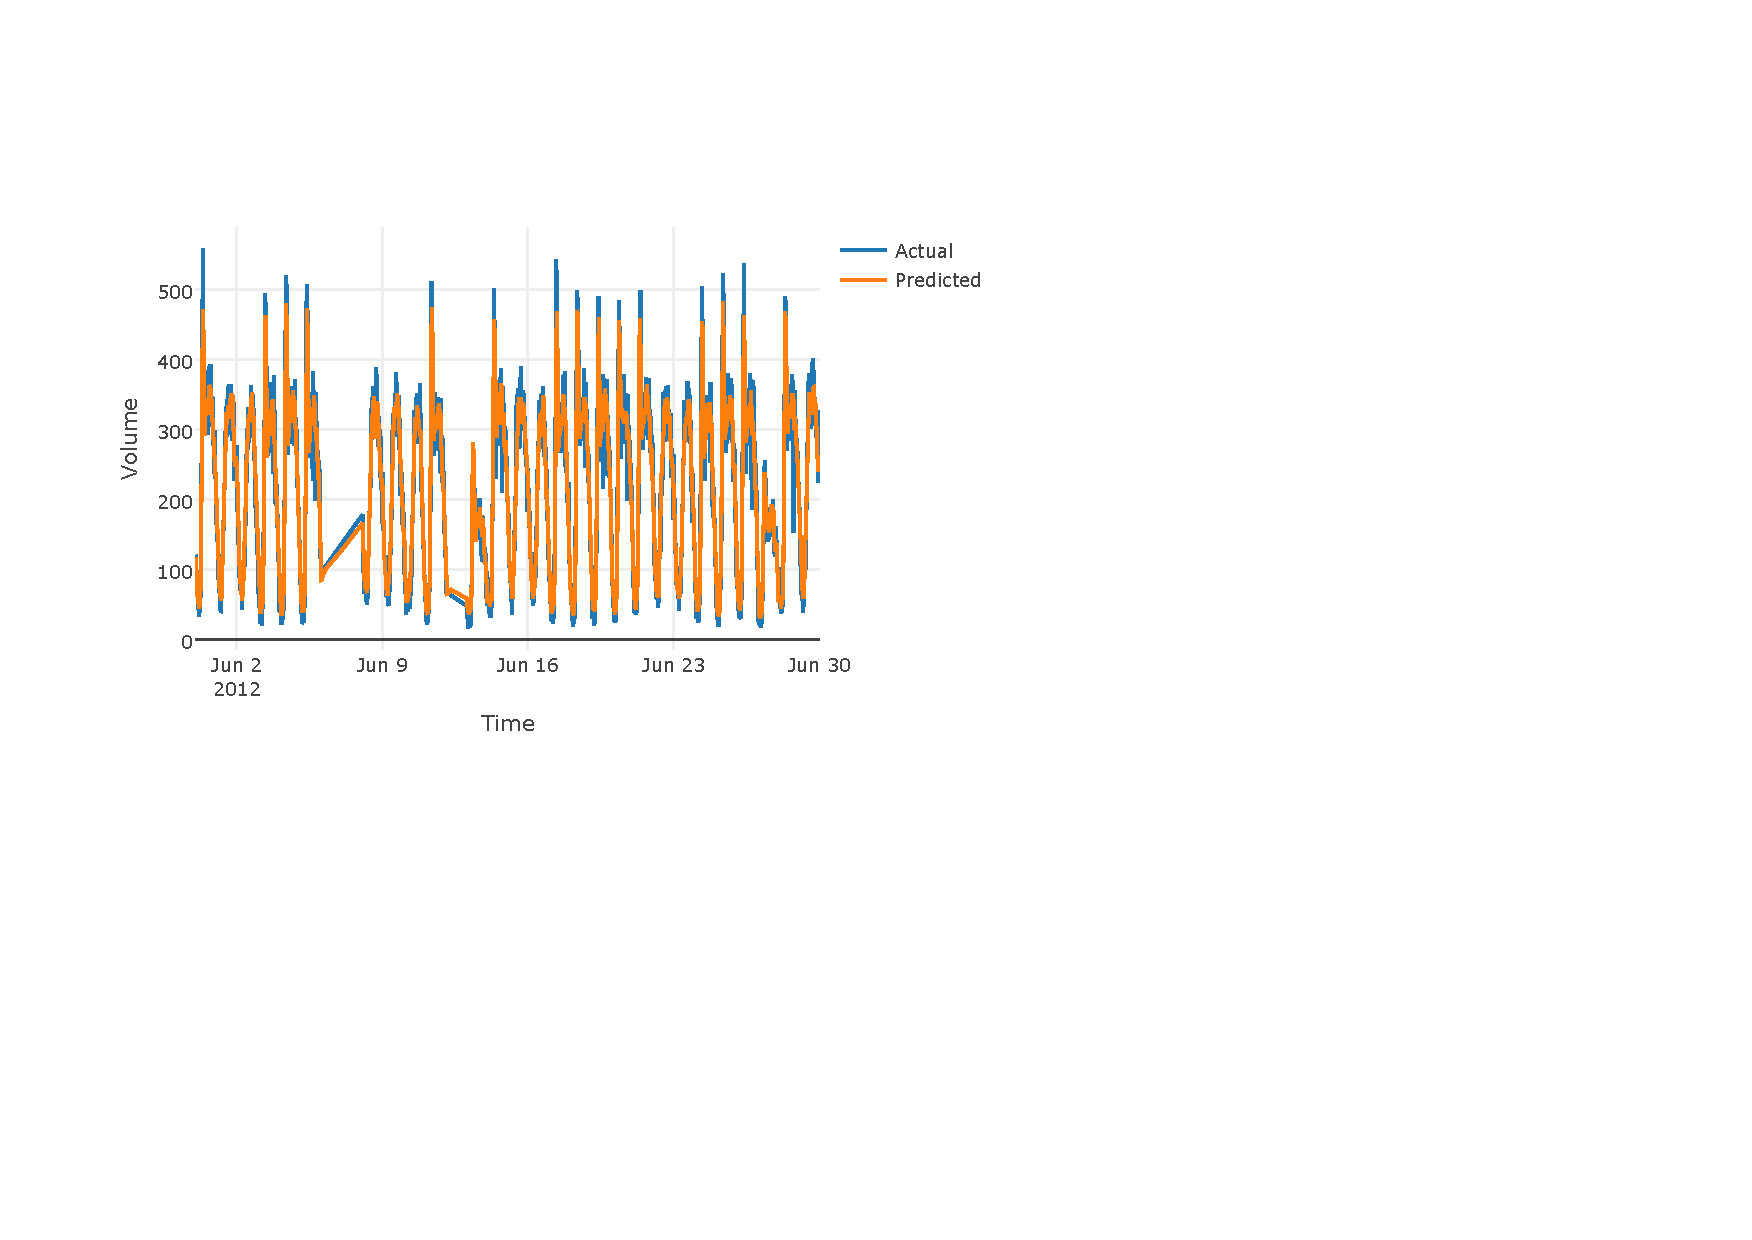
\includegraphics[width=0.4\textwidth]{Plots/gru-multi1.pdf}
    \label{fig:GRUMultiActualPredicted1}}
    \qquad
    \subfloat[RNN - multiple locations][RNN - multiple locations]{
    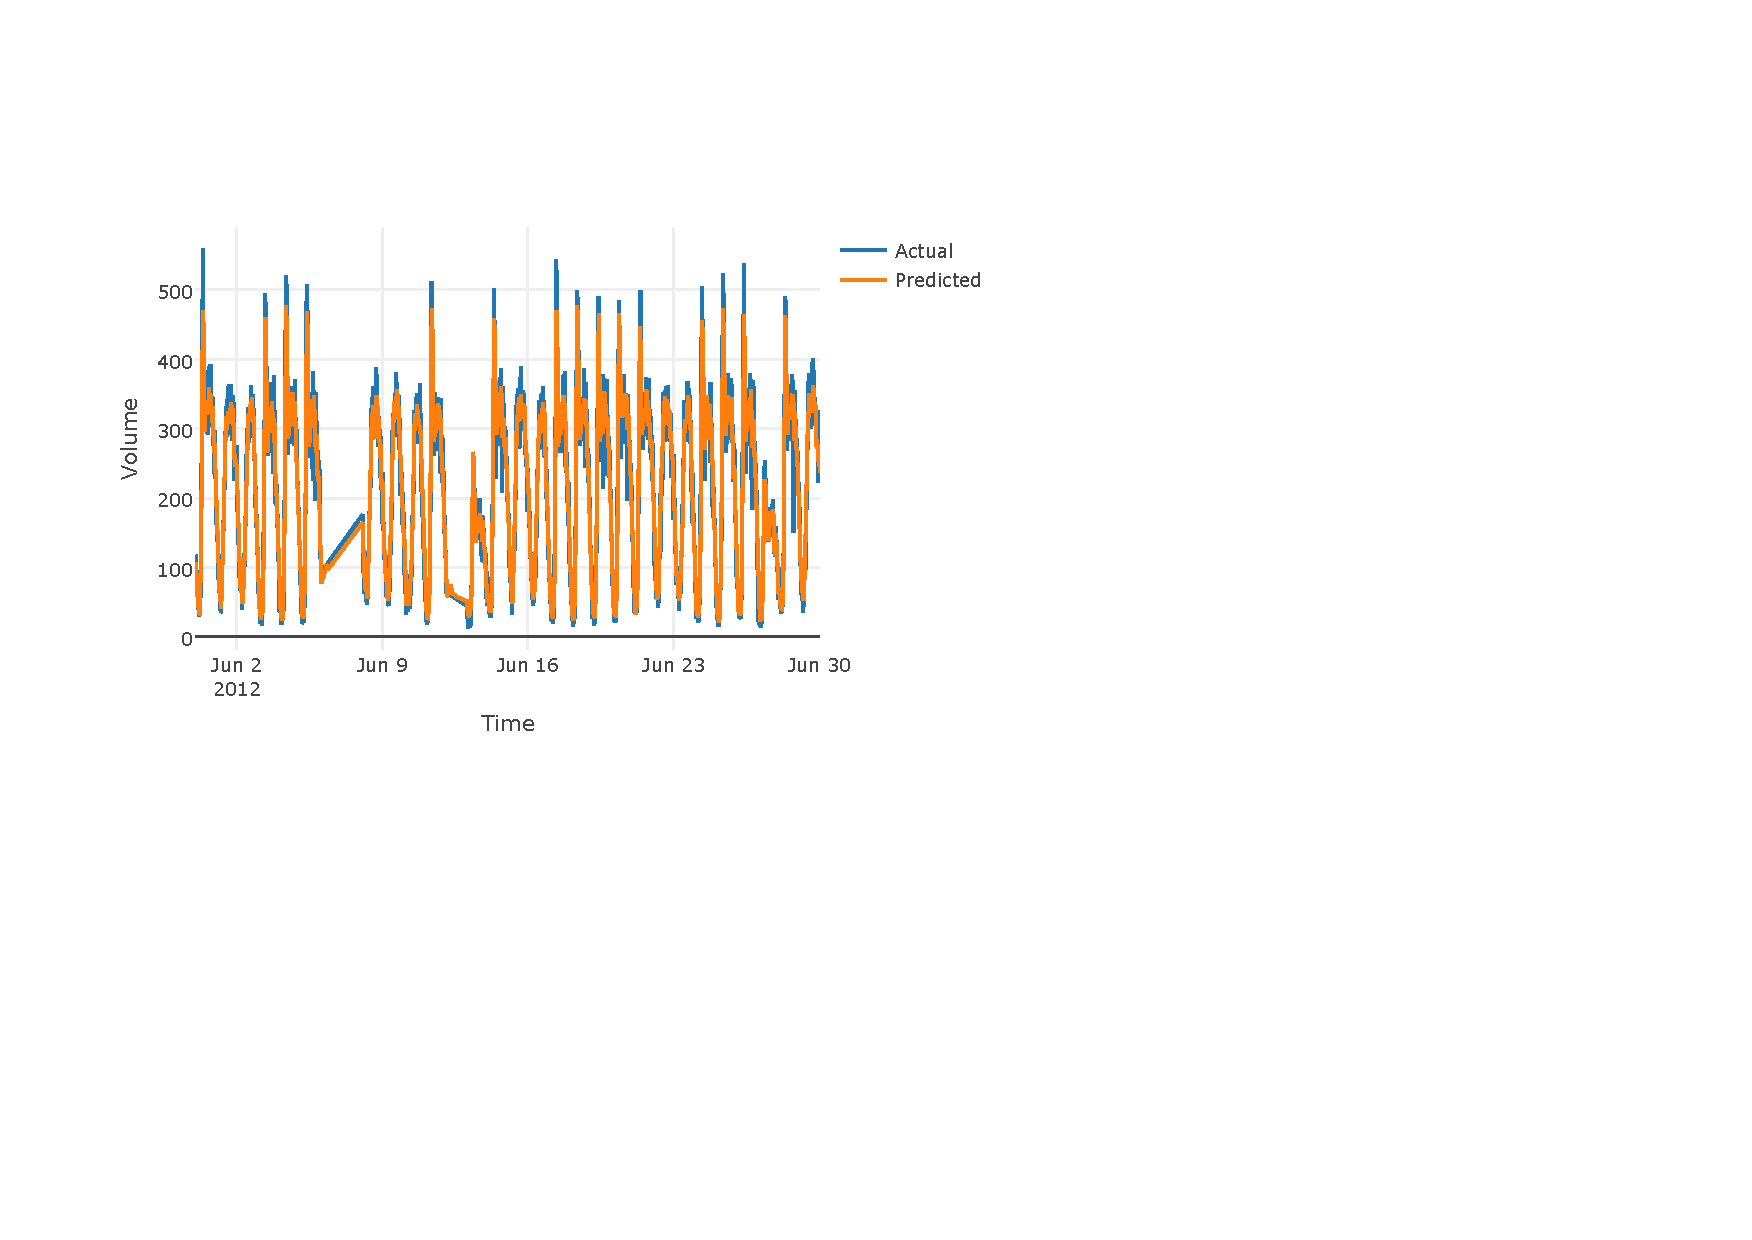
\includegraphics[width=0.4\textwidth]{Plots/rnn-multi1.pdf}
    \label{fig:RNNMultiActualPredicted1}}

    \caption[Actual vs Predictions, using deep networks]{Actual vs Predictions - using three deep
    neural networks (LSTM, GRU and Simple RNN). The top three are results for the single homogeneous
    road segment when using data from that location only while the bottom three are results for the
    single homogeneous road segment when data from neighbouring locations (\ref{fig:ExperimentRegion})
    were also used . The plots show the actual vs predictions (15 mins) for the month of June 2012.}
    \label{fig:deepNNModels}
\end{figure}

\section{Comparisons}

\subsection{Prediction accuracies}
For model comparison we used three accuracy measures - mean absolute error (MAE), root mean squared
error (RMSE) and mean absolute percentage error (MAPE). In below sections we briefly describe
the accuracy measures.

For defining the accuracy measures let us denote $x_{i}$ be the $i^{th}$ observation and
$\hat{x}_{i}$ be the prediction of $x_{i}$.

\textbf{Scale-dependent errors}
The prediction error is simply given by $e_{i} = x_{i} - \hat{x}_{i}$, which is in the same scale
as of the original data. So accuracy measures that depend on $e_{i}$ are scale dependent and can
not be used across multiple series on different scales. The two most used scale-dependent
accuracy measures are mean absolute error and root mean squared error defined as below

    \begin{equation}
        MAE = mean(\abs{e_{i}})
    \end{equation}
    \begin{equation}
        RMSE = \sqrt{mean(e^{2}_{i})}
    \end{equation}

MAE is easy to understand and popular in usage when using a single dataset.

\textbf{Percentage errors}
Percentage errors are scale-independent and thus used across multiple datasets on different
scales. The percentage error is given by $p_{i} = 100*e_{i}/x_{i}$. The most commonly used
percentage measure is Mean Absolute Percentage Error (MAPE) which is given by the below formula
    \begin{equation}
        MAPE = mean(\abs{p_{i}})
    \end{equation}

There are however few shortcomings of the MAPE, for instance when $x_{i}$ is 0 or very large.
Another shortcoming is that they put heavier penalty on negative error values than positive error
values.

\begin{figure}[htbp]
    \centering
    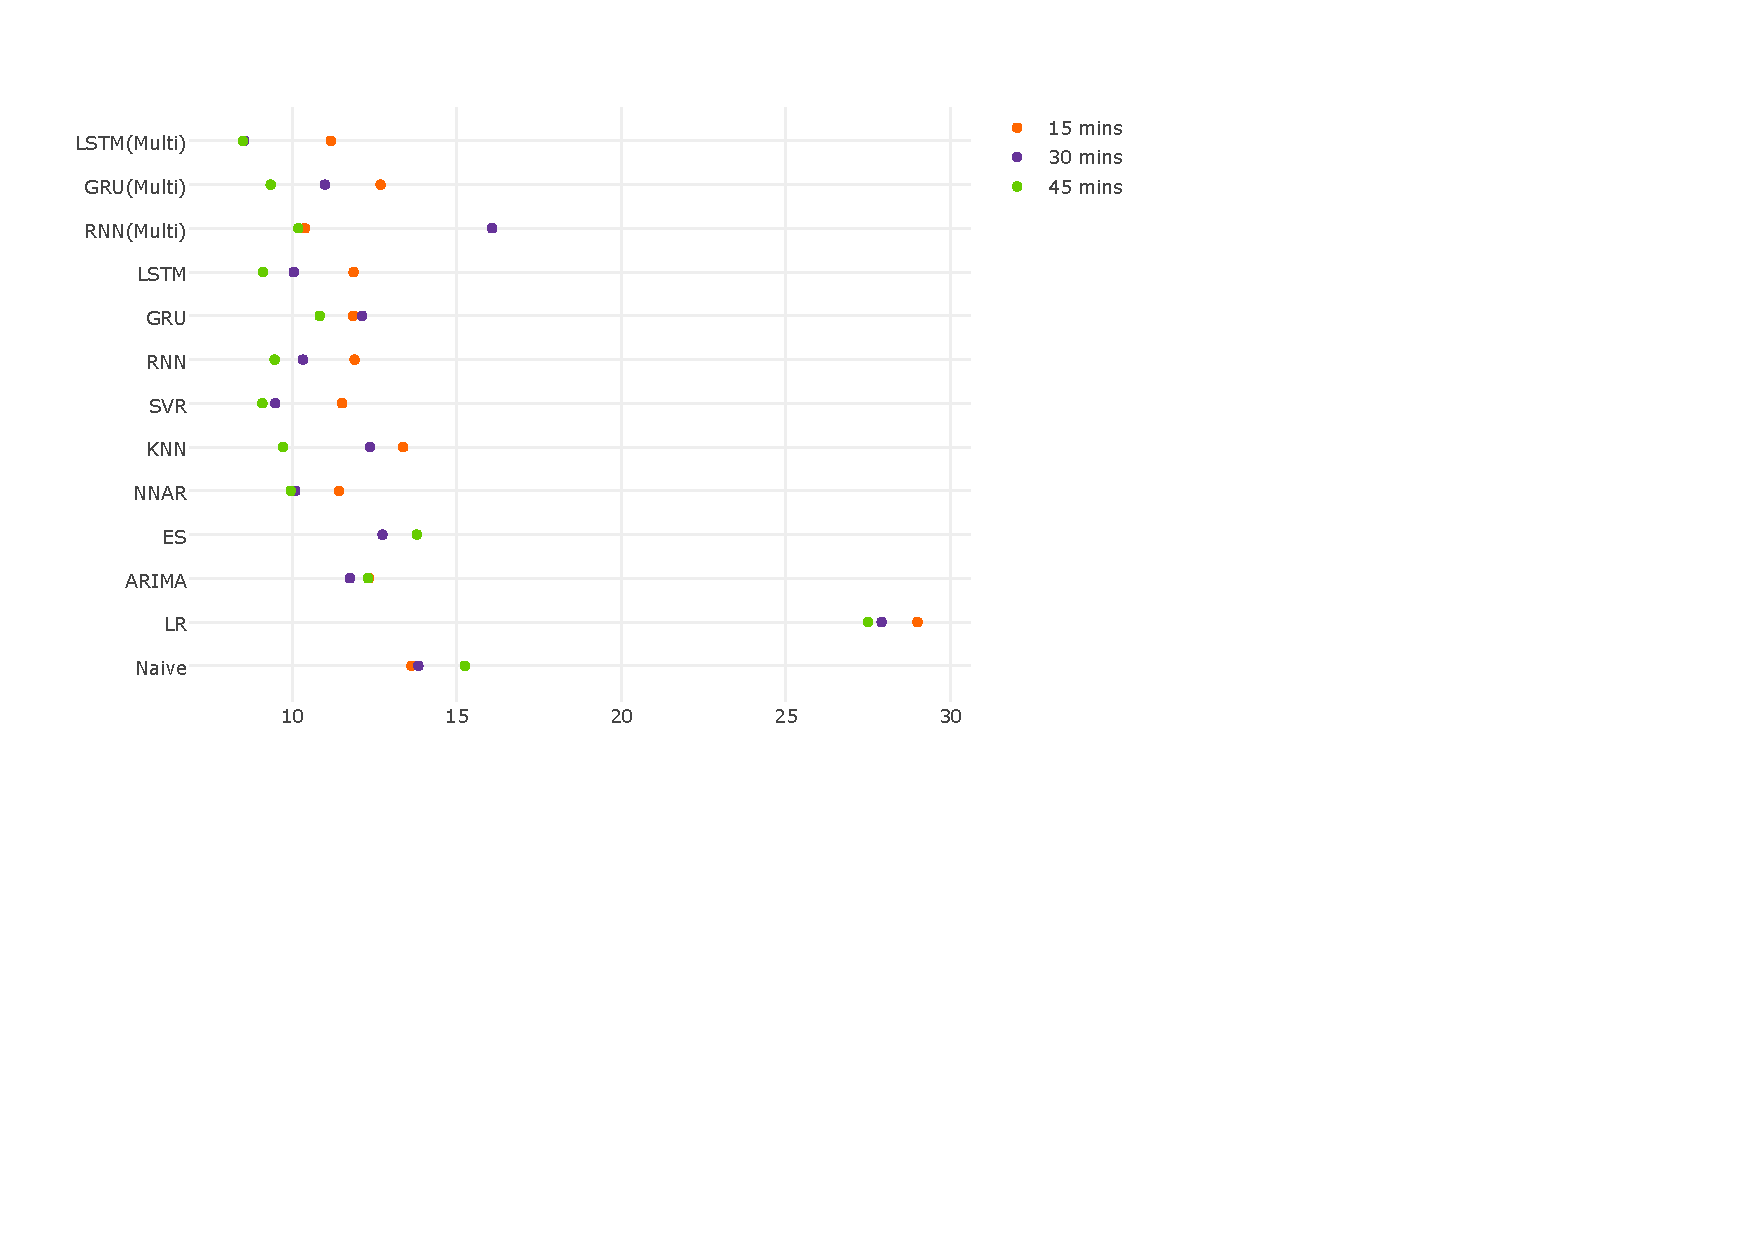
\includegraphics[width=0.7\textwidth]{Plots/mape-errors.pdf}
    \rule{35em}{0.5pt}
    \caption[MAPE scores for the methods]{MAPE scores for the methods}
    \label{fig:mapeErrors}
\end{figure}

In table \ref{table:accuracyScores}, the accuracies are presented in terms of the above mentioned
error measures for the methods presented in this experiment. The error measures are presented for
the predictions for 1 step-ahead (15-minutes), 2 steps-ahead (30-minutes) and 3-steps ahead (45-minutes).

The accuracy of the naive method for 15-minutes predictions was about 86.4\%, which is very good
considering no computations are required.
The linear regression has the worst performance among all the methods, with only 71\% of accuracy for
15-minutes predictions, including the baseline naive method. All other methods had better performance
than the naive method. Among the exisiting methods, neural network autoregression has the best
performance with an accuracy of about 89.6\%.

Overall the best accuracies in both one-step and multi-steps predictions were achieved by the deep
LSTM and GRU networks with multivariate modelling. For 15-minutes prediction, the best performance
was achieved by the deep GRU (multivariate) with about 89.3\% accuracy, while for 30 and 45-minutes
predictions the best performance was by the LSTM (multivariate) network with accuracies of about
91.6\% and 92.7\%.
In figure \ref{fig:mapeErrors}, the mean absolute percentage errors of all the methods for 15, 30
and 45 minutes predictions are plotted.

The advantage of the deep networks used in the multivariate settings is that the predictions of
all the 11 locations were done at the same time. In table \ref{table:locationErrors}, we present the
error measures for these locations of the deep LSTM network.

\begin{table}
    \begin{tabular}{c}
        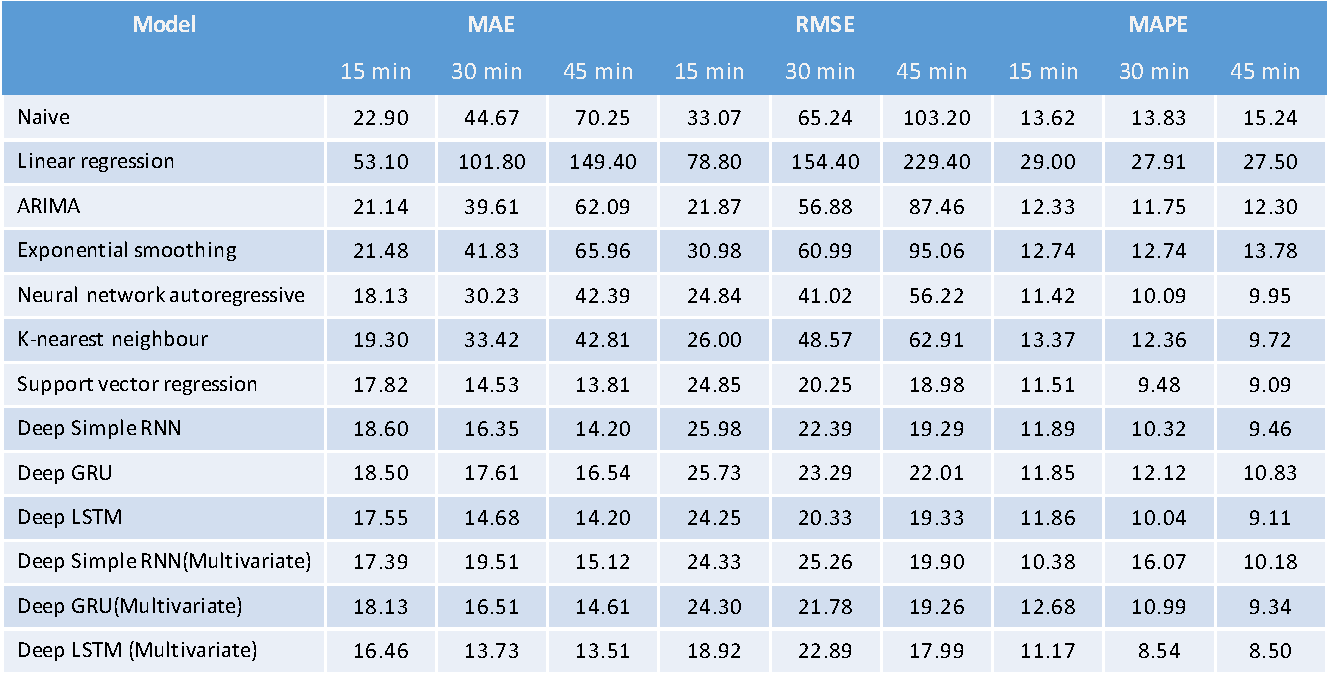
\includegraphics[width=\textwidth,height=\textheight,keepaspectratio]{Figures/errors-table.pdf}
    \end{tabular}
    \caption[Model comparisons]{Accuracy measures for the evaluated models. The scores are
    calculated for prediction horizon of 15, 30 and 45 minutes. Mean 15-minutes traffic
    volume is 224.10}
    \label{table:accuracyScores}
\end{table}

\begin{table}
    \begin{tabular}{c}
        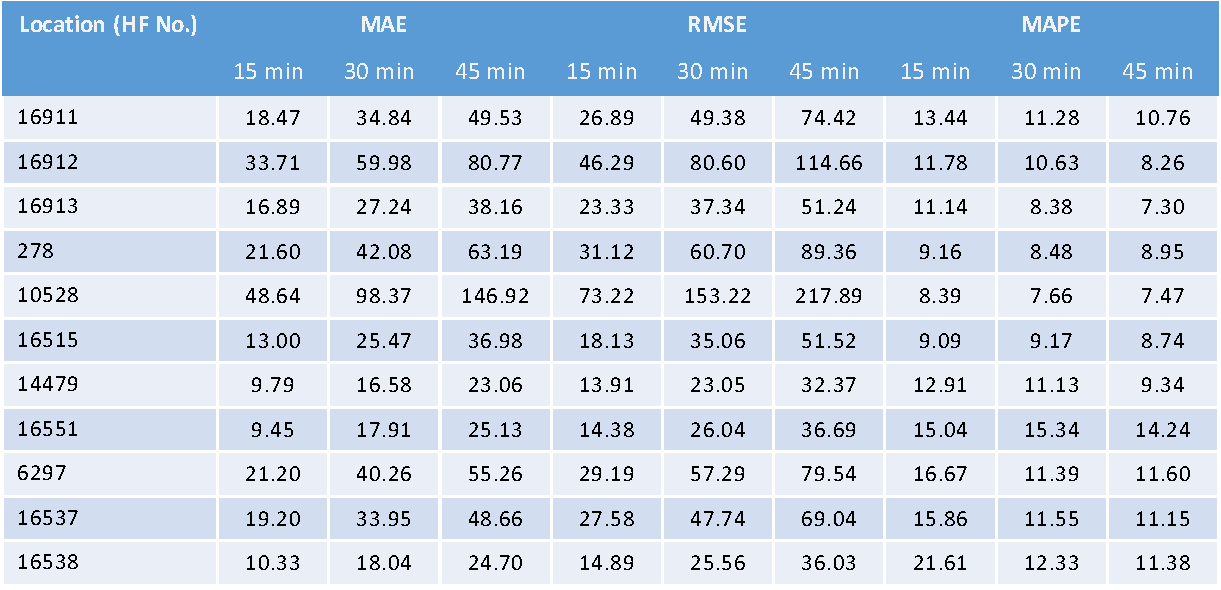
\includegraphics[width=\textwidth,height=\textheight,keepaspectratio]{Figures/errors-locations-table.pdf}
    \end{tabular}
    \caption[Simultaneous predictions across all the locations]{Simultaneous predictions across all
    the locations using the deep LSTM network. The network models the spatio-temporal characteristics
    from the traffic volume data.}
    \label{table:locationErrors}
\end{table}

\subsection{Computational time}

\begin{figure}[htbp]
    \centering
    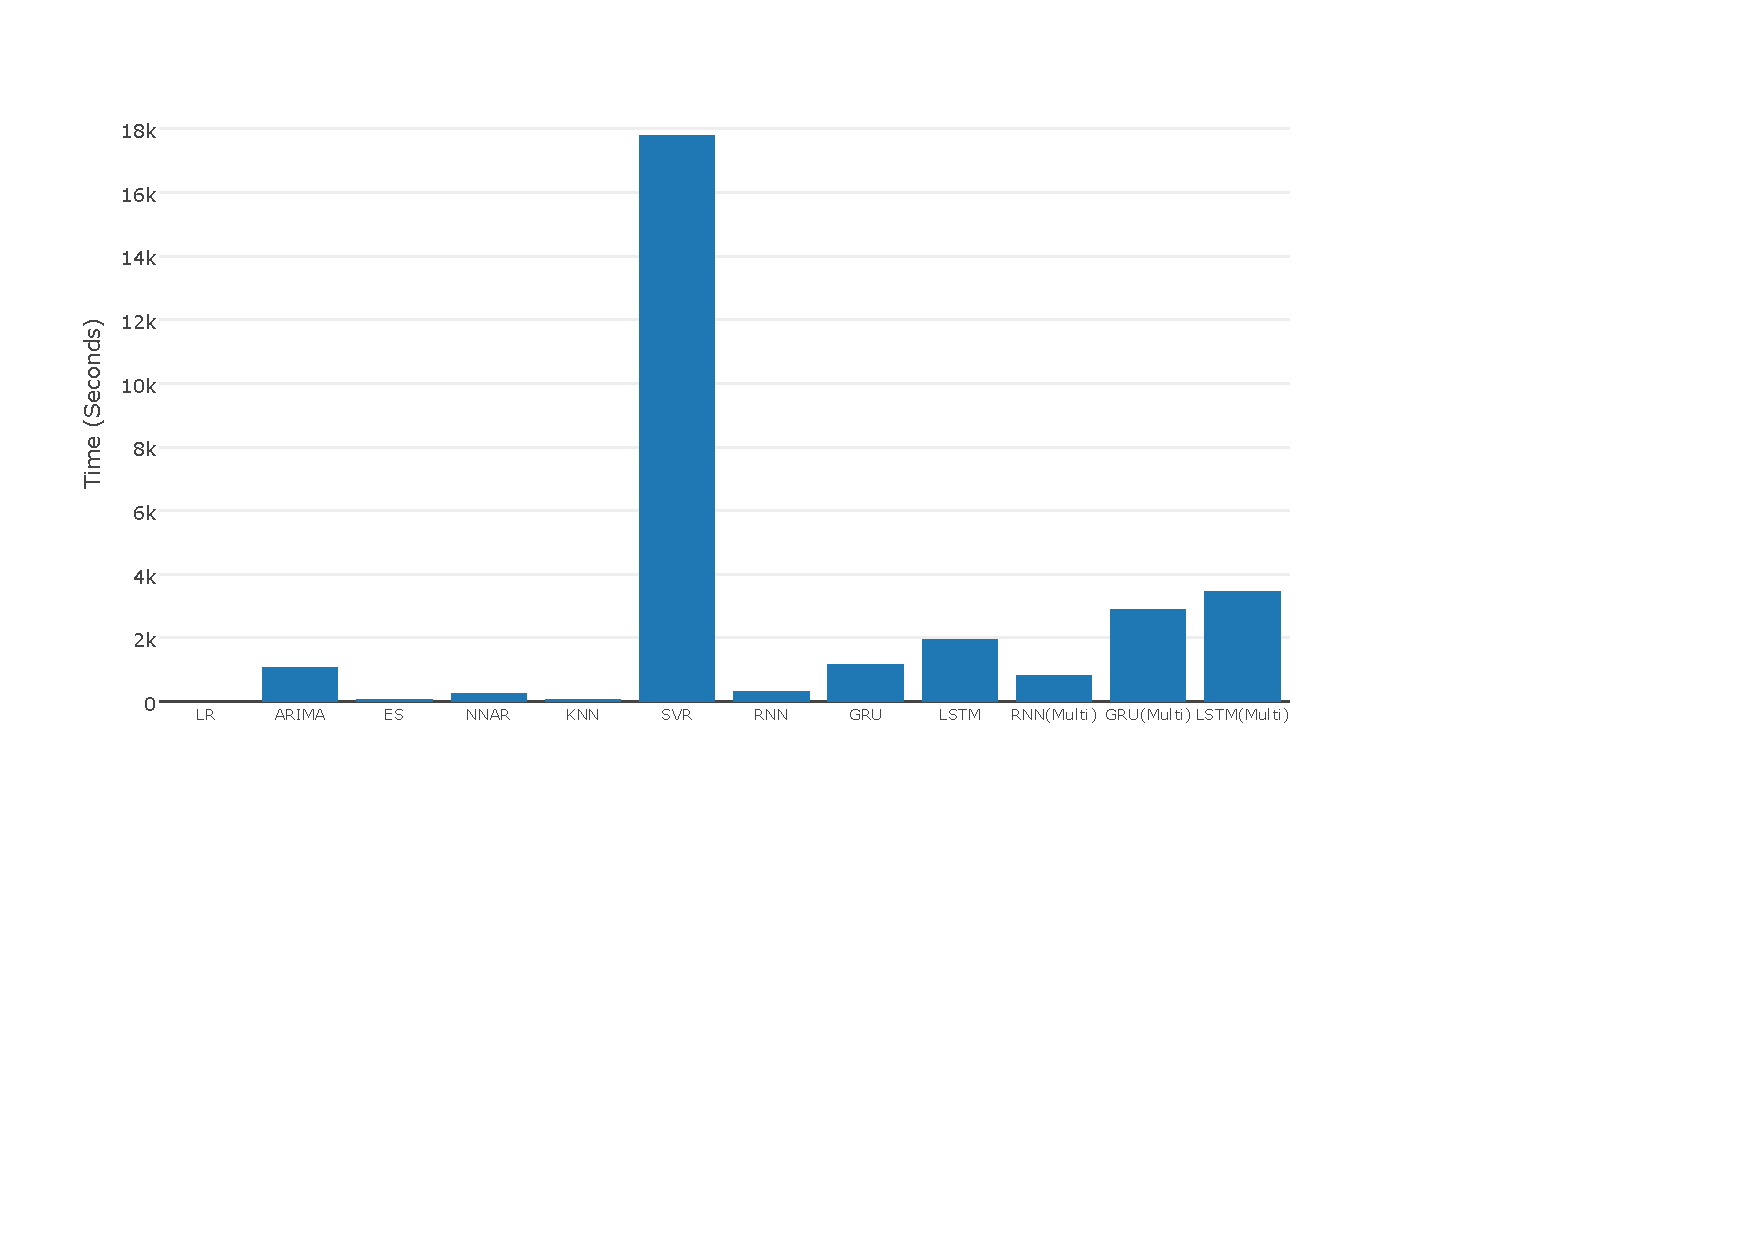
\includegraphics[width=0.7\textwidth]{Plots/training-time.pdf}
    \rule{35em}{0.5pt}
   \caption[Comparison of training time of the models]{Comparison of training time of the models}
    \label{fig:trainingTime}
\end{figure}

For all these experiments we used a home computer with Intel i7-4770 CPU, 16GB RAM, GeForce GTX 960
GPU. The operating system used was Ubuntu 14.04 and for data processing and modelling we used R and
Python languages. The training time of all the above mentioned models (except Naive)  are shown in
the figure \ref{fig:trainingTime}. However not all of the algorithms were used optimised to reduce
the training time, so the figures could vary in small amounts.


In this chapter we presented the results of our experiments in short term traffic prediction using
several models. We compared the results and found that the performance of deep neural networks
outperform all the existing methods.
% Chapter 6

\chapter{Conclusions and Future Directions} % Main chapter title

\label{Chapter6} % For referencing the chapter elsewhere, use \ref{Chapter6}

% This is for the header on each page - perhaps a shortened title
\lhead{Chapter 6. \emph{Conclusions and Future Directions}}

% Quotation
``Everything should be made as simple as possible but not simpler."

\begin{flushright}
Albert Einstein
\end{flushright}

%---------------------------------------------------------------------------------------------------
%	CONTENT
%---------------------------------------------------------------------------------------------------

\section{Conclusions}

In this work, we reviewed the existing literature on short term traffic prediction and proposed
how a long short term momory recurrent neural network can be used for this task.


\section{Future works}


%---------------------------------------------------------------------------------------------------
%	THESIS CONTENT - APPENDICES
%---------------------------------------------------------------------------------------------------

\addtocontents{toc}{\vspace{2em}} % Add a gap in the Contents, for aesthetics

\appendix % Cue to tell LaTeX that the following 'chapters' are Appendices

% Include the appendices of the thesis as separate files from the Appendices folder Uncomment the
% lines as you write the Appendices

% Appendix A

\chapter{Appendix Title Here} % Main appendix title

\label{AppendixA} % For referencing this appendix elsewhere, use \ref{AppendixA}

\lhead{Appendix A. \emph{Appendix Title Here}} % This is for the header on each page - perhaps a shortened title

Write your Appendix content here.
%\input{Appendices/AppendixB}
%\input{Appendices/AppendixC}

\addtocontents{toc}{\vspace{2em}} % Add a gap in the Contents, for aesthetics

\backmatter

%---------------------------------------------------------------------------------------------------
%	BIBLIOGRAPHY
%---------------------------------------------------------------------------------------------------

\label{Bibliography}

\lhead{\emph{Bibliography}} % Change the page header to say "Bibliography"

\bibliographystyle{apalike} % Use the "apalike" BibTeX style for formatting the Bibliography

% The references (bibliography) information are stored in the file named "Bibliography.bib"
\bibliography{Bibliography}

\nocite{*}

\end{document}
